\documentclass[11pt,a4paper]{article}

\usepackage[utf8]{inputenc}
\usepackage[T1]{fontenc}
\usepackage{lmodern}
\DeclareRobustCommand{\code}[1]{\texttt{\detokenize{#1}}}
\usepackage{geometry}
\geometry{top=2.2cm, bottom=2.5cm, left=2.2cm, right=2.2cm}
\usepackage{amsmath,amssymb,amsfonts}
\usepackage{graphicx}
\usepackage{booktabs}
\usepackage[expansion=false]{microtype}
\usepackage{xcolor}
\usepackage{hyperref}
\usepackage{listings}
\usepackage{fancyhdr}
\usepackage{titlesec}
\usepackage{enumitem}
\usepackage{tabularx}
\usepackage{tcolorbox}
\usepackage{float}
\usepackage{caption}
\usepackage{subcaption}

% Color palette definitions
\definecolor{astraBlue}{RGB}{24, 76, 120}
\definecolor{astraDark}{RGB}{30, 41, 59}
\definecolor{astraCyan}{RGB}{14, 116, 144}
\definecolor{astraGreen}{RGB}{22, 101, 52}
\definecolor{astraRed}{RGB}{153, 27, 27}
\definecolor{codeBg}{RGB}{248, 250, 252}
\definecolor{codeBorder}{RGB}{226, 232, 240}
\definecolor{darkTerminalBg}{RGB}{24, 24, 24}

\hypersetup{
    colorlinks=true,
    linkcolor=astraBlue,
    citecolor=astraCyan,
    urlcolor=astraBlue
}

% Header and Footer
\pagestyle{fancy}
\setlength{\headheight}{15pt}
\addtolength{\topmargin}{-3pt}
\fancyhf{}
\fancyhead[L]{\textsc{ASTRA: Autonomous CPU/GPU Job Scheduler}}
\fancyhead[R]{\thepage}
\fancyfoot[C]{\footnotesize Systems Design \& Operating Systems Comprehensive Technical Report}
\renewcommand{\headrulewidth}{0.6pt}
\renewcommand{\footrulewidth}{0.4pt}

% Section styling
\titleformat{\section}{\color{astraDark}\normalfont\Large\bfseries}{\thesection}{1em}{}[\titlerule]
\titleformat{\subsection}{\color{astraBlue}\normalfont\large\bfseries}{\thesubsection}{1em}{}
\titleformat{\subsubsection}{\color{astraCyan}\normalfont\normalsize\bfseries}{\thesubsubsection}{1em}{}

% Listings configuration
\lstset{
    backgroundcolor=\color{codeBg},
    basicstyle=\ttfamily\footnotesize,
    breaklines=true,
    frame=single,
    rulecolor=\color{codeBorder},
    numbers=left,
    numberstyle=\tiny\color{gray},
    numbersep=7pt,
    tabsize=2,
    showstringspaces=false,
    keywordstyle=\color{astraBlue}\bfseries,
    commentstyle=\color{gray}\itshape,
    stringstyle=\color{astraGreen}
}

\begin{document}

% ==============================================================================
% TITLE & METADATA
% ==============================================================================
\begin{titlepage}
    \centering
    \vspace*{1.0cm}
    
    {\Huge \textbf{\color{astraDark} ASTRA: Autonomous Compute Scheduler}}\\[0.4cm]
    {\LARGE \textbf{\color{astraBlue} Systems Engineering, Mathematical Modeling, and Verification of a CPU/GPU Process Scheduler in C++20 for Linux Environments}}\\[1.2cm]
    
    \rule{\linewidth}{1.2pt}\\[0.5cm]
    
    \textbf{Course Domain:} Advanced Operating Systems $\cdot$ Systems Programming $\cdot$ Parallel Scheduling\\
    \textbf{Target Platform:} Ubuntu 24.04.1 LTS on WSL2 (Linux Kernel 6.18) $\cdot$ POSIX.1-2008 Standard\\
    \textbf{Host Hardware:} x86\_64 (16 Logical Cores) $\cdot$ NVIDIA GeForce RTX 3050 Laptop GPU (4 GB VRAM)\\
    \textbf{Implementation Language:} Modern ISO C++20 (GCC 13.3.0, Ninja, CMake 3.28)\\
    \textbf{Date of Audit \& Release:} October 2026\\[0.5cm]
    \rule{\linewidth}{1.2pt}
    
    \vspace{1.5cm}
    
    \begin{tcolorbox}[colback=codeBg,colframe=astraBlue,title=\textbf{Executive Abstract}]
    This document presents the complete systems engineering specification, mathematical formalisms, architectural decomposition, and empirical benchmarks for \textbf{ASTRA} (Autonomous System for Task Scheduling \& Resource Allocation). ASTRA is a production-grade, terminal-native compute scheduler engineered from first principles in C++20. Operating at the boundary between userspace process management and kernel resource abstractions, ASTRA manages concurrent POSIX workloads, enforces multi-resource admission limits (CPU core slots, RAM limits, NVIDIA GPU VRAM), arbitrates scheduling policies (FCFS, Strict Priority, Priority Aging, and SJF), coordinates full-duplex Inter-Process Communication via UNIX domain stream socketpairs (\code{AF_UNIX}), guarantees crash-consistency via atomic write-sync-rename protocols, detects DAG workflow cycles with 3-color DFS, and demonstrates explainable deadlock recovery through Dijkstra's classical Banker's Algorithm. The system has achieved a 100\% passing verification score across all 10 automated test suites with zero zombie process leaks.
    \end{tcolorbox}
    
    \vfill
    
    {\small Authoritative Technical Reference \& Architecture Manual $\cdot$ Release Milestone v0.1.0-alpha}
\end{titlepage}

\tableofcontents
\newpage

% ==============================================================================
% SECTION 1: INTRODUCTION & PROBLEM FORMULATION
% ==============================================================================
\section{Introduction \& System Problem Formulation}

\subsection{Kernel Scheduling vs. Userspace Compute Schedulers}
In contemporary computing systems, a fundamental distinction exists between operating system kernel schedulers and userspace compute schedulers:
\begin{enumerate}[leftmargin=*]
    \item \textbf{Kernel-Level CPU Schedulers (e.g., Linux CFS):} The Completely Fair Scheduler (CFS) inside the Linux kernel operates at microsecond quantum granularities. Its primary objective is fair distribution of hardware execution time among competing threads and processes using red-black tree data structures tracking virtual runtime (\code{vruntime}). It possesses no domain awareness regarding application-level job deadlines, multi-step Directed Acyclic Graph (DAG) dependencies, or multi-resource co-allocation.
    \item \textbf{Userspace Compute Schedulers (e.g., ASTRA):} Schedulers such as Slurm, Kubernetes, or ASTRA operate at the macroeconomic macroscopic job level (milliseconds to hours). A compute scheduler owns process orchestration: it decides \textit{when} a workload is admitted, \textit{which} dedicated child worker process executes it, \textit{how much} CPU and GPU capacity is reserved, and \textit{how} dependency cascades and hardware failures are mitigated.
\end{enumerate}

\subsection{Core Challenges in Compute Scheduling}
Designing a robust compute scheduler on POSIX systems requires overcoming several classic operating systems challenges:
\begin{itemize}[leftmargin=*]
    \item \textbf{Convoy Effect in First-Come First-Served (FCFS):} When long-running CPU-bound tasks arrive ahead of short, interactive tasks, average queuing delays escalate dramatically.
    \item \textbf{Starvation in Strict Priority Schemes:} High-priority tasks arriving in bursts can permanently deny execution slots to low-priority tasks (priority inversion and starvation).
    \item \textbf{Resource Contention \& Deadlocks:} When multiple workloads compete for distinct resources (e.g., CPU slots and GPU VRAM), uncoordinated resource allocation can lead to circular wait conditions and permanent deadlocks.
    \item \textbf{Inter-Process Communication Bottlenecks \& Leaks:} IPC via non-blocking pipes or socketpairs must handle partial reads, OS signals (\code{EINTR}), framing overhead, and buffer overflow without deadlock or descriptor leaks.
    \item \textbf{Zombie Process Accumulation:} Exited child workloads remain in the kernel process table as defunct zombies unless cleanly reaped via \code{waitpid(2)} or asynchronous \code{SIGCHLD} handlers.
    \item \textbf{Crash Consistency:} Abnormal worker termination must be isolated; intermediate computation must be cooperatively checkpointed to non-volatile storage without corruption.
\end{itemize}

\begin{figure}[H]
    \centering
    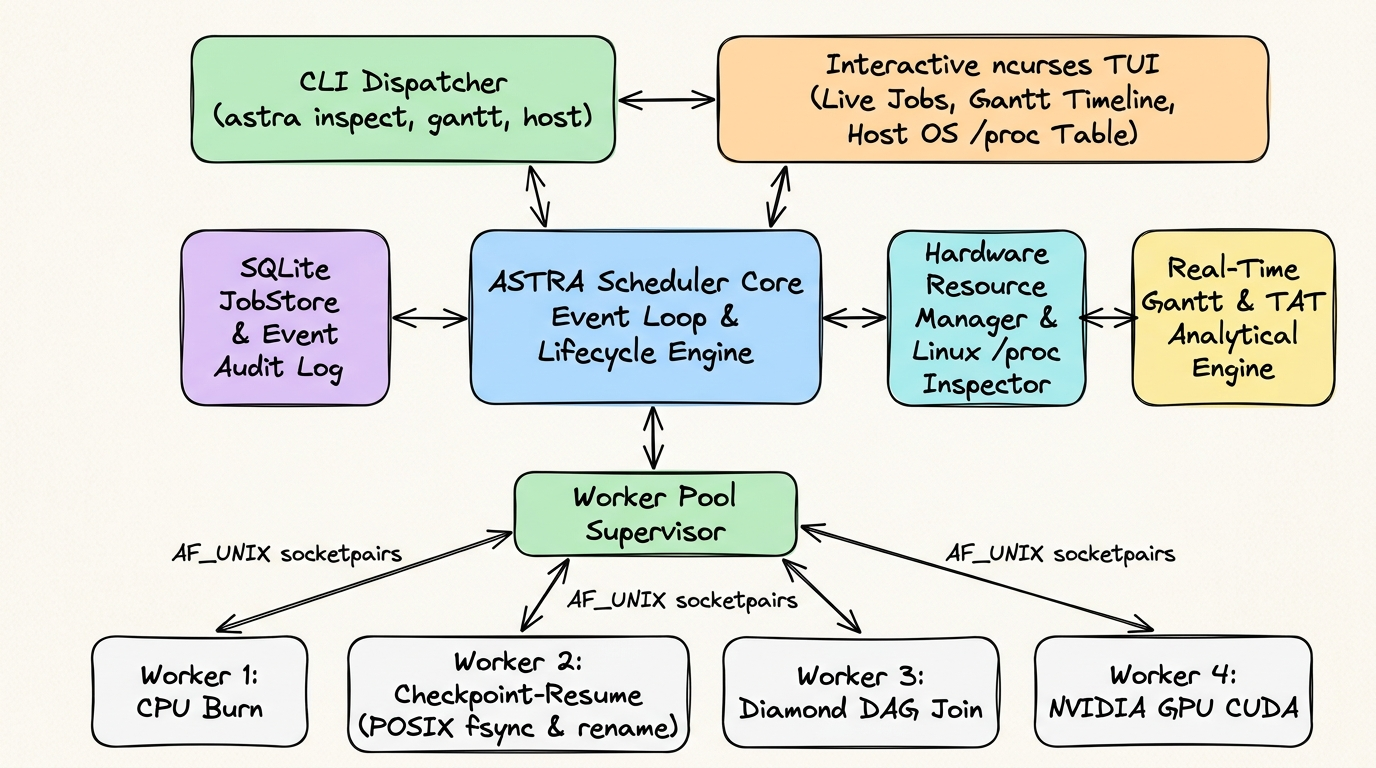
\includegraphics[width=0.98\textwidth]{figures/excalidraw_system_arch.jpg}
    \caption{\textbf{ASTRA End-to-End System Architecture (Excalidraw Design).} Depicting the decoupled layers: CLI/TUI interfaces, Single-Threaded Scheduler Core Event Loop, SQLite Storage Engine, Resource Manager, Worker Manager Pool Supervisor, and Child Workloads communicating over \texttt{AF\_UNIX} Socketpairs.}
    \label{fig:arch}
\end{figure}

% ==============================================================================
% SECTION 2: OPERATING SYSTEM MECHANISMS & POSIX PRIMITIVES
% ==============================================================================
\section{Operating System Mechanics \& POSIX Primitives}

ASTRA is built upon strict POSIX standards (POSIX.1-2008) executed within Ubuntu 24.04 LTS running on Microsoft WSL2 with direct NVIDIA driver virtualization.

\subsection{Process Creation \& Isolation (\texttt{fork} and \texttt{execvp})}
Child workers and application workloads are spawned using the canonical POSIX process instantiation pipeline:
\begin{lstlisting}[language=C++]
pid_t pid = fork();
if (pid == 0) {
    // Child process context: configure file descriptors and signal masks
    dup2(pipe_out[1], STDOUT_FILENO);
    dup2(pipe_err[1], STDERR_FILENO);
    close(pipe_out[0]); close(pipe_out[1]);
    
    // Execute workload binary without invoking a shell interpreter
    execvp(argv[0], const_cast<char* const*>(argv.data()));
    _exit(127); // execvp failure exit
}
\end{lstlisting}
By directly utilizing \code{execvp(3)} rather than \code{system(3)} or shell command strings, ASTRA achieves immunity from arbitrary shell injection attacks, malicious metacharacter interpretation, and command substitution vulnerabilities.

\subsection{Elimination of Zombie Processes (\texttt{waitpid} with \texttt{WNOHANG})}
When a child process terminates, its exit status and resource accounting statistics remain in the kernel process descriptor table until consumed by its parent. If the parent neglects to reap the child, the process transitions to a \code{ZOMBIE} (\code{[defunct]}) state. ASTRA completely eliminates zombie accumulation through non-blocking status polling in the worker event loop:
\begin{equation}
    \code{waitpid}(-1, \&\text{status}, \code{WNOHANG})
\end{equation}
When \code{waitpid} returns $W > 0$, ASTRA inspects the macros \code{WIFEXITED(status)} and \code{WEXITSTATUS(status)} to record legitimate termination, or \code{WIFSIGNALED(status)} and \code{WTERMSIG(status)} to diagnose process termination via asynchronous signals (such as \code{SIGSEGV} or \code{SIGKILL}).

\subsection{Inter-Process Communication (\texttt{socketpair(AF\_UNIX, SOCK\_STREAM, 0)})}
Rather than relying on un-interleaved pipes or shared memory with risky user-space mutexes, ASTRA establishes a dedicated full-duplex UNIX domain stream socketpair per worker supervisor:
\begin{lstlisting}[language=C++]
int fds[2];
if (socketpair(AF_UNIX, SOCK_STREAM, 0, fds) != 0) {
    throw SystemException("socketpair creation failed", errno);
}
// fds[0] retained by Scheduler Daemon; fds[1] inherited by Child Worker
\end{lstlisting}
UNIX domain sockets run entirely within the kernel's virtual memory subsystem without network stack overhead, yielding microsecond latency and full-duplex protocol framing.

\begin{figure}[H]
    \centering
    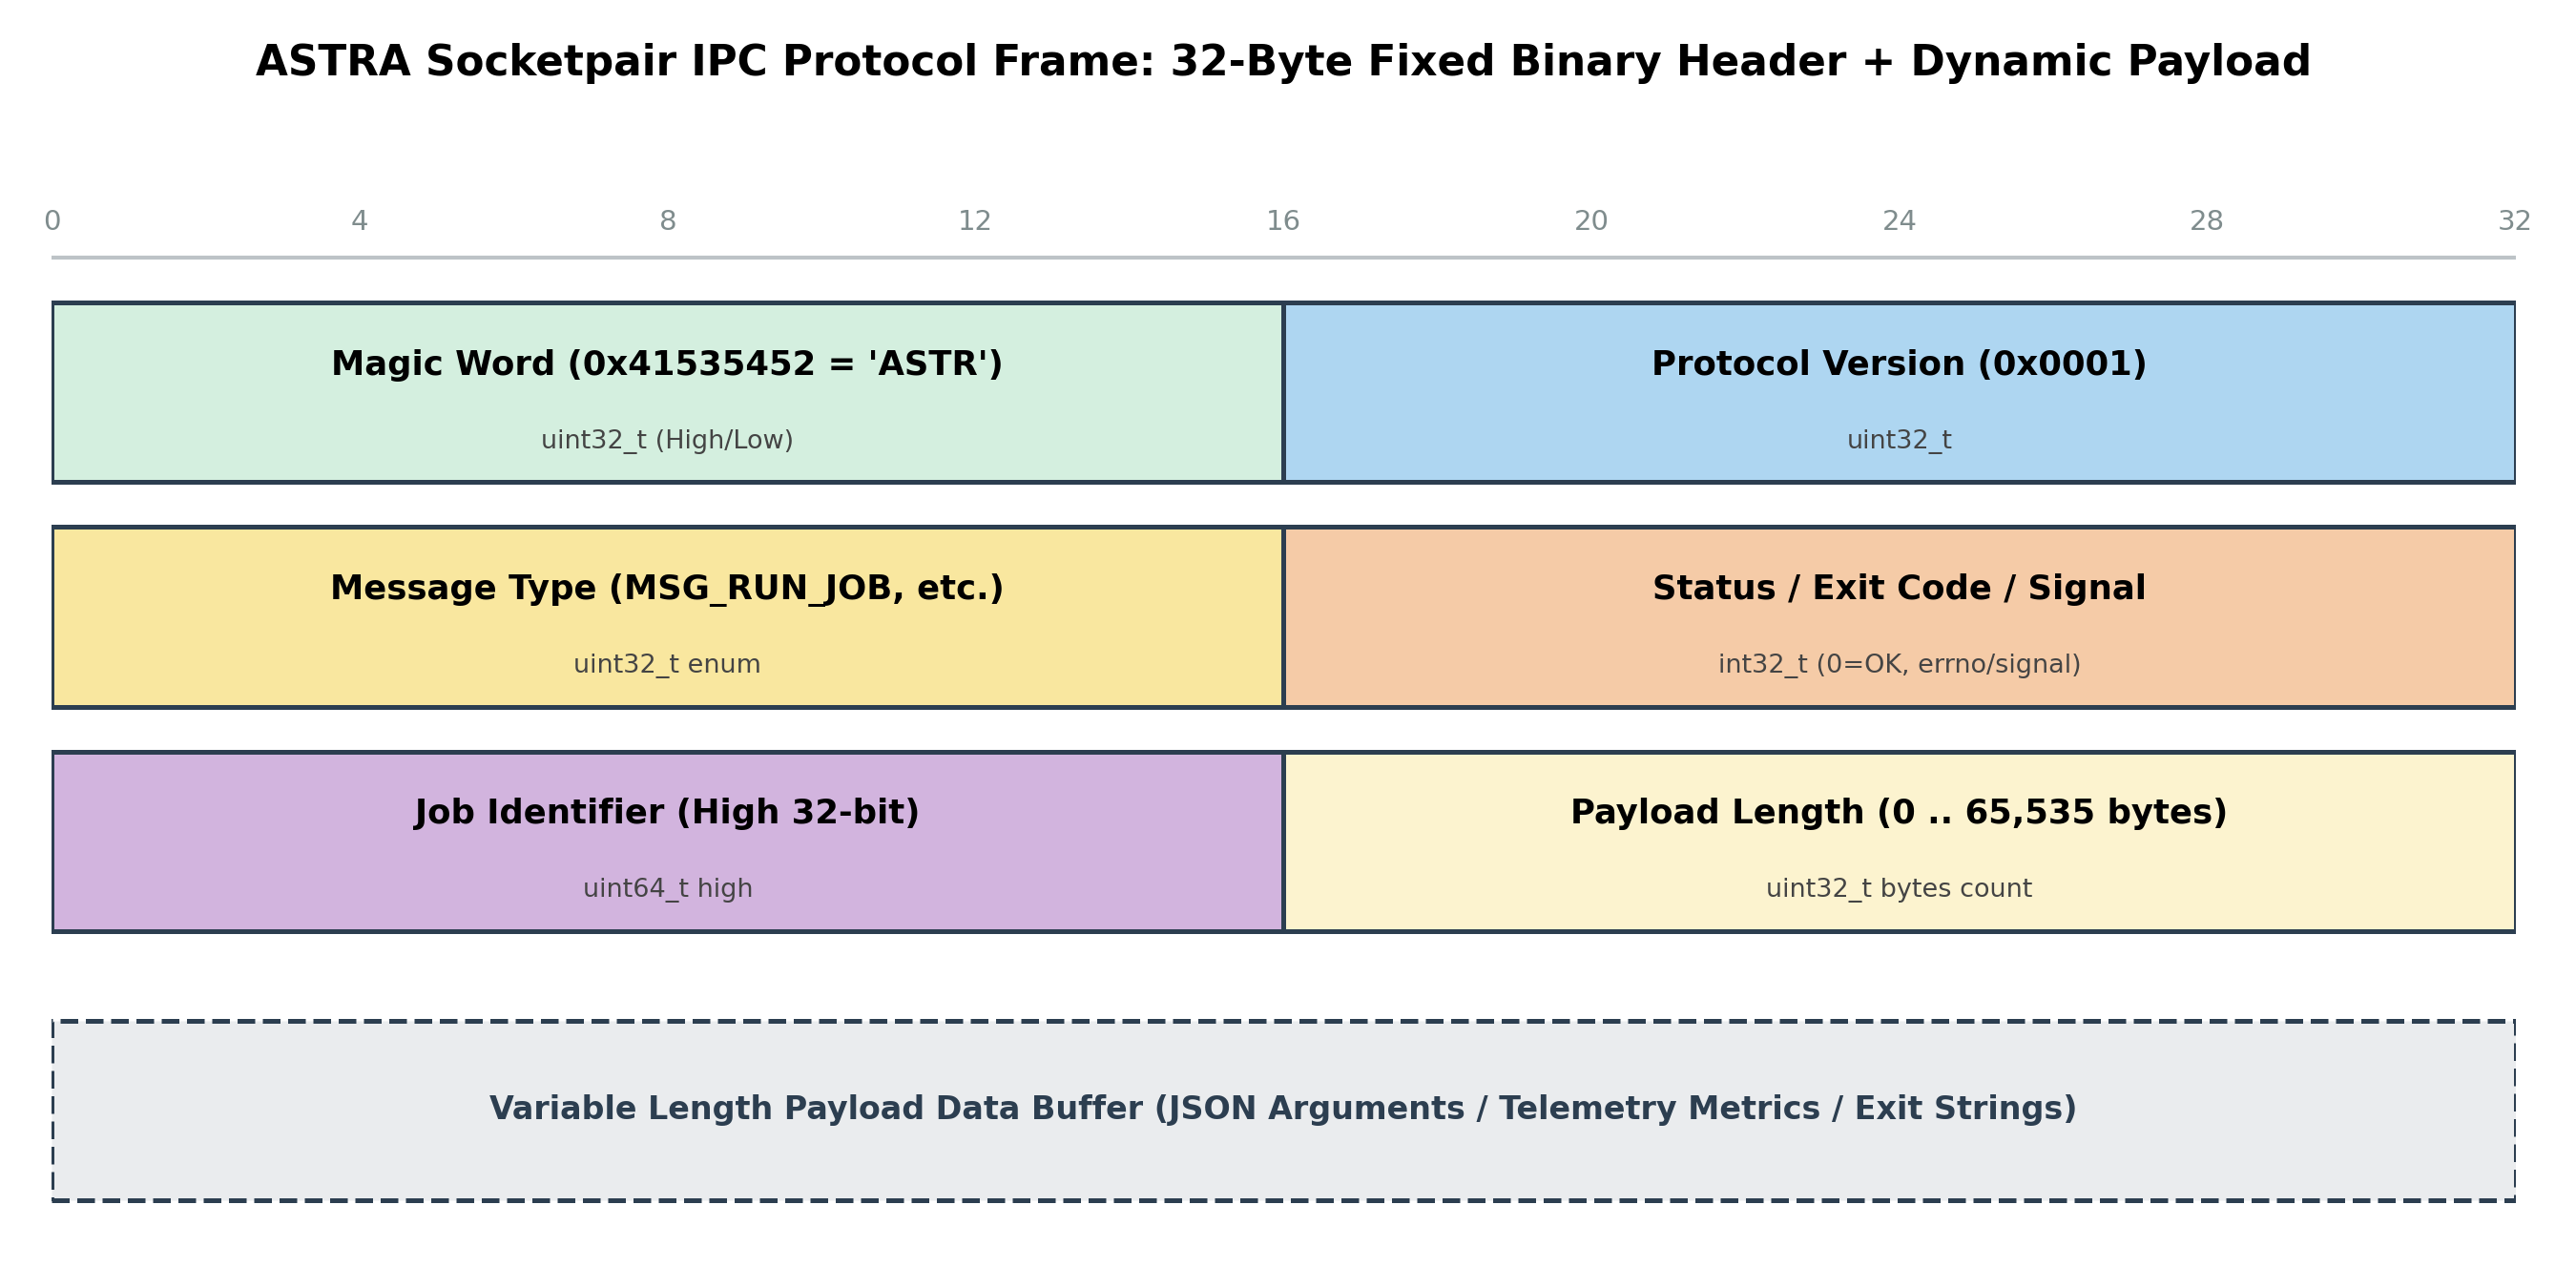
\includegraphics[width=0.88\textwidth]{figures/figure3_ipc_protocol.png}
    \caption{\textbf{ASTRA Binary IPC Packet Structure.} 32-byte fixed-width binary header encapsulating magic token \texttt{0x41535452}, message type, job ID, status/signal code, and payload length followed by variable-length JSON arguments.}
    \label{fig:ipc}
\end{figure}

\subsection{Atomic Checkpointing via POSIX \texttt{fsync} and \texttt{rename(2)}}
A critical flaw in naive file-based persistence is crash corruption: if a process crashes while actively writing a checkpoint file, the file is left truncated and corrupted. ASTRA enforces the ACID Write-Sync-Rename protocol:
\begin{enumerate}
    \item The workload writes intermediate state to a temporary file: \code{checkpoint_path + ".tmp"}.
    \item The process calls \code{fsync(fileno(fp))}, forcing the OS page cache buffers to flush directly to physical non-volatile storage.
    \item The process invokes \code{rename(tmp_path, checkpoint_path)}.
\end{enumerate}
Under POSIX kernel specifications, \code{rename(2)} is guaranteed to be an atomic filesystem metadata transaction. The old valid checkpoint is replaced by the new valid checkpoint instantaneously; an incomplete write can never overwrite valid state.

\begin{figure}[H]
    \centering
    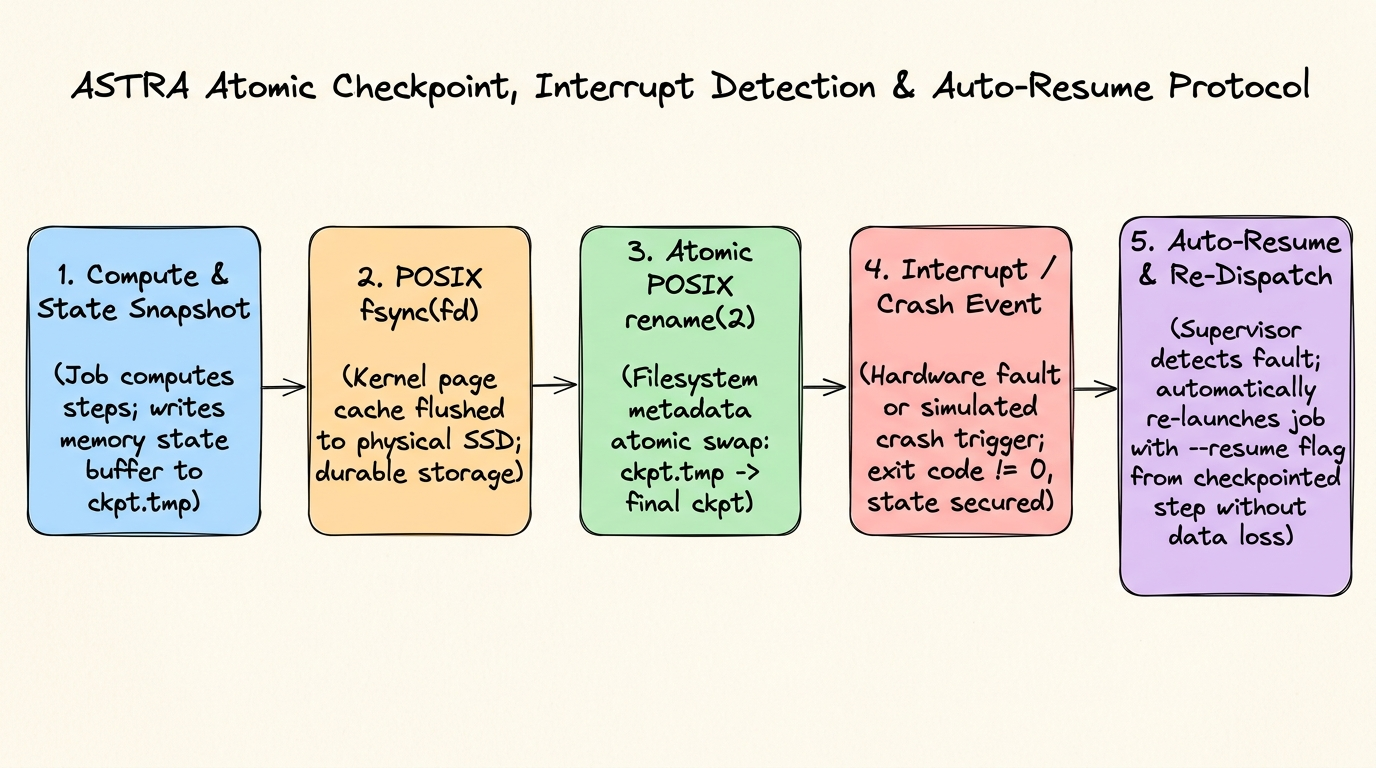
\includegraphics[width=0.96\textwidth]{figures/excalidraw_checkpoint_flow.jpg}
    \caption{\textbf{Atomic Checkpoint-Resume Protocol (Excalidraw Architecture Design).} Step-by-step lifecycle ensuring zero corruption on unannounced process crash through atomic POSIX write-sync-rename primitives.}
    \label{fig:ckpt}
\end{figure}

% ==============================================================================
% SECTION 3: SYSTEM ARCHITECTURE & FILE-BY-FILE SPECIFICATION
% ==============================================================================
\section{System Architecture \& Comprehensive File-by-File Specification}

The ASTRA codebase adheres strictly to clean architecture principles and separation of concerns. Every file, directory, and class in the project is detailed below.

\subsection{Subsystem Directory Organization}
\begin{table}[H]
\centering
\small
\begin{tabularx}{\textwidth}{l p{4.2cm} X}
\toprule
\textbf{Directory} & \textbf{Component Role} & \textbf{Architectural Responsibility} \\
\midrule
\code{include/astra/} & Public Header Interfaces & C++20 declarations, enum types, RAII wrappers, and API contracts. \\
\code{src/resources/} & Configuration \& Resources & Physical telemetry parsers (\code{/proc/meminfo}), GPU query, limits. \\
\code{src/storage/}   & Relational Persistence   & SQLite3 ACID engine, migration v1 schemas, indexed lookups. \\
\code{src/cli/}       & Interaction Engine       & Tokenizer, path security validators, CLI handler, and REPL. \\
\code{src/ipc/}       & Inter-Process Comm       & Framed 32-byte binary UNIX socketpair communications. \\
\code{src/worker/}    & Worker Supervision       & Child process lifecycle, signal cancellation escalation, reaping. \\
\code{src/scheduler/} & Scheduler Core           & Single-threaded event loop, FCFS/Priority/Aging/SJF algorithms. \\
\code{src/tui/}       & Terminal Dashboard       & Full-screen \code{ncurses} terminal user interface and telemetry snapshots. \\
\code{src/workflow/}  & DAG Workflow Engine      & Kahn's topological sort, 3-color DFS cycle detector, multi-branch join. \\
\code{src/deadlock/}  & Deadlock Laboratory      & Dijkstra's Banker's algorithm, Wait-For Graph (WFG), victim selection. \\
\code{src/checkpoint/}& Crash Consistency        & Atomic file serialization, \code{fsync} page cache flush, POSIX rename. \\
\code{src/replay/}    & Deterministic Replay     & Audit event timeline reconstruction, delta time indexing, table output. \\
\code{src/benchmark/} & Policy Benchmark Suite   & Multi-slot discrete-event simulation evaluating scheduling algorithms. \\
\code{workloads/}     & Synthetic Workloads      & CPU burn, parallel sum, intentional crash, and checkpointable sum. \\
\code{cuda/}          & GPU Workloads            & CUDA vector addition kernel with seamless host fallback. \\
\code{tests/}         & Automated Verification   & Unit, integration, and regression suites for all 10 milestones. \\
\code{scripts/}       & Automation Tooling       & End-to-end verification demo script (\code{demo.sh}). \\
\bottomrule
\end{tabularx}
\caption{\textbf{ASTRA Project Directory Layout and Component Roles.}}
\label{tab:dirs}
\end{table}

\subsection{Exhaustive File Functionality Registry}

\subsubsection{Core Domain \& Persistence}
\begin{itemize}[leftmargin=*]
    \item \textbf{\code{include/astra/version.hpp}:} Stores semantic version string (\code{0.1.0-alpha}) and ASCII visual banner.
    \item \textbf{\code{include/astra/job_state.hpp}:} Defines the 12-state \code{JobState} enum and central transition validation table (\code{is_valid_transition()}). Enforces deterministic FSM evolution.
    \item \textbf{\code{include/astra/job.hpp}:} Implements the core domain entities: \code{ResourceRequest} (CPU slots, RAM, GPU requirements), \code{JobAttempt} (timestamps, exit status, worker PID), and \code{Job} (unique ID, priority, dependency list, deadline, retry counter). Includes complete bidirectional JSON serialization via \code{nlohmann::json}.
    \item \textbf{\code{include/astra/event.hpp}:} Defines the 17 \code{EventType} audit markers (e.g., \code{JOB_SUBMITTED}, \code{JOB_QUEUED}, \code{JOB_STARTED}, \code{DEADLOCK_DETECTED}, \code{RECOVERY_APPLIED}, \code{JOB_COMPLETED}) ensuring immutable auditability.
    \item \textbf{\code{include/astra/config.hpp} \& \code{src/resources/config.cpp}:} Defines \code{AstraConfig} parameter validation (worker pool size, max CPU slots, default policy, aging interval, DB path) and JSON configuration loader.
    \item \textbf{\code{include/astra/job_store.hpp} \& \code{src/storage/job_store.cpp}:} High-performance SQLite3 storage abstraction implementing PIMPL idiom. Automatically applies Schema Migration v1 creating tables: \code{jobs}, \code{job_dependencies}, \code{attempts}, \code{workers}, \code{events}, and \code{workflows}. Provides prepared statements for all operations with atomic transactions.
\end{itemize}

\begin{figure}[H]
    \centering
    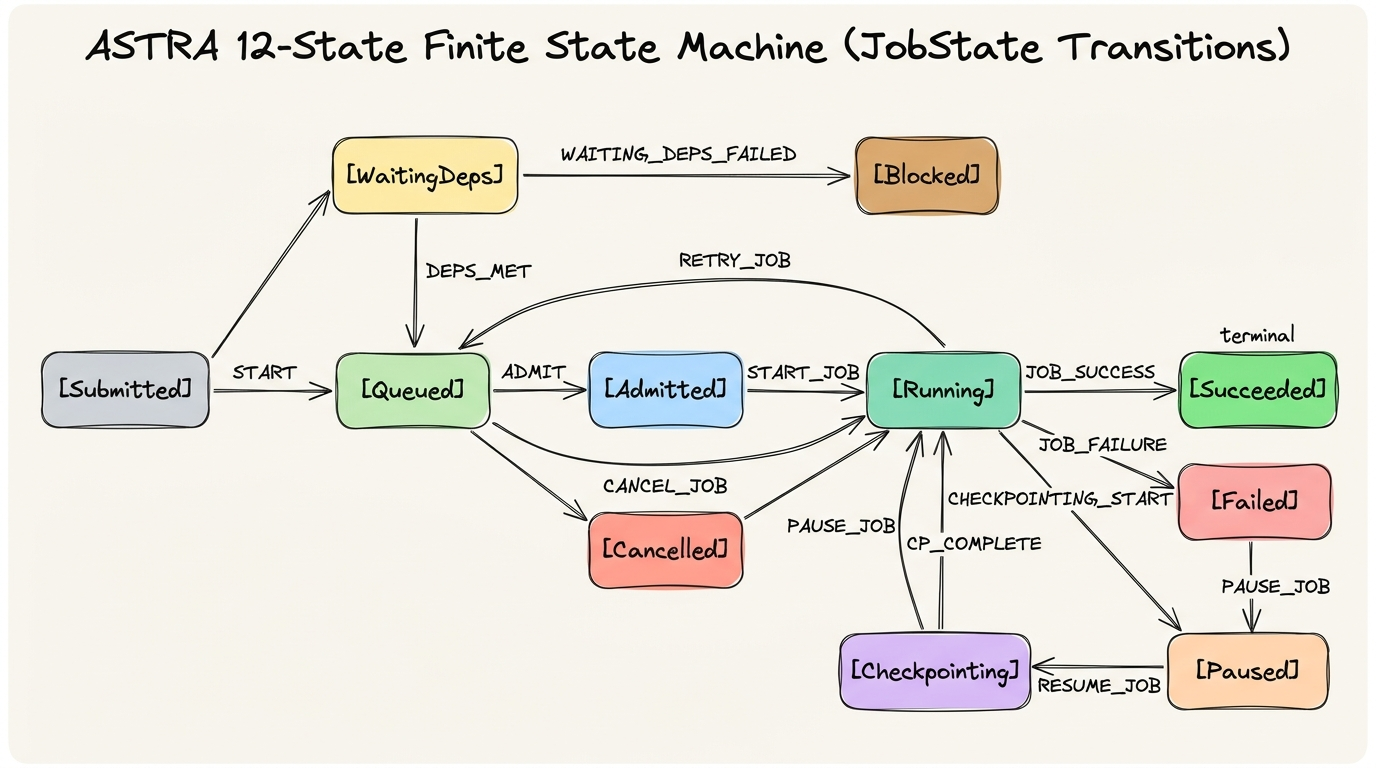
\includegraphics[width=0.96\textwidth]{figures/excalidraw_state_machine.jpg}
    \caption{\textbf{ASTRA 12-State Finite State Machine (Excalidraw Architecture Design).} Central validation logic enforces legal state transitions, rejecting illegal jumps and recording transition audit events.}
    \label{fig:fsm}
\end{figure}

\subsubsection{CLI, Tokenization, and REPL}
\begin{itemize}[leftmargin=*]
    \item \textbf{\code{include/astra/command.hpp}:} Strongly typed CLI command representation using C++20 \code{std::variant} over structures (\code{SubmitCommand}, \code{PsCommand}, \code{InspectCommand}, \code{CancelCommand}, \code{WorkflowCommand}, \code{ReplayCommand}, \code{BenchmarkCommand}, etc.).
    \item \textbf{\code{include/astra/command_parser.hpp} \& \code{src/cli/command_parser.cpp}:} Implements robust command tokenization handling escaped quotes, whitespace, and command-line options. Enforces path security allowlists, rejecting directory traversal attempts (\code{".."}) and shell chaining characters (\code{";"}, \code{"\&"}, \code{"|"}).
    \item \textbf{\code{include/astra/cli_handler.hpp} \& \code{src/cli/cli_handler.cpp}:} Dispatches parsed commands to underlying storage and scheduler layers; hosts the interactive REPL prompt (\code{astra> }) with tabular formatting.
\end{itemize}

\subsubsection{Worker Pool Supervision \& IPC}
\begin{itemize}[leftmargin=*]
    \item \textbf{\code{include/astra/ipc_channel.hpp} \& \code{src/ipc/ipc_channel.cpp}:} Wraps \code{AF_UNIX} socketpair in \code{IpcChannel} with RAII \code{UniqueFd}. Handles partial reads/writes, signal interruptions (\code{EINTR}), and message framing.
    \item \textbf{\code{include/astra/worker.hpp} \& \code{src/worker/worker.cpp}:} Child worker supervisor process loop. Receives \code{MSG_RUN_JOB}, forks workload, redirects stdout/stderr into non-blocking pipes, monitors child execution, and streams progress back to the parent.
    \item \textbf{\code{include/astra/worker_manager.hpp} \& \code{src/worker/worker_manager.cpp}:} Oversees pool of child worker processes. Implements graceful cancellation escalation: issues \code{SIGTERM}, awaits grace period, escalates to \code{SIGKILL} if unresponsive, reaps terminated children via \code{waitpid(WNOHANG)}, and automatically restores crashed worker slots.
\end{itemize}

\subsubsection{Scheduler Core, Policies, and Admission Control}
\begin{itemize}[leftmargin=*]
    \item \textbf{\code{include/astra/scheduling_policy.hpp} \& \code{src/scheduler/scheduling_policy.cpp}:} Polymorphic engine implementing \code{FcfsPolicy}, \code{PriorityPolicy}, \code{PriorityAgingPolicy}, and \code{SjfPolicy}.
    \item \textbf{\code{include/astra/resource_manager.hpp} \& \code{src/resources/resource_manager.cpp}:} Tracks logical resource reservations (CPU core slots, RAM limits, GPU availability). Parses Linux telemetry from \code{/proc/meminfo} and interfaces with the NVIDIA driver via \code{nvidia-smi} / NVML. Guarantees exact-once release semantics.
    \item \textbf{\code{include/astra/scheduler.hpp} \& \code{src/scheduler/scheduler.cpp}:} Central single-threaded event loop. Dispatches admitted jobs to idle workers, processes completed workload events, and evaluates dependency unblocking.
\end{itemize}

\subsubsection{Terminal User Interface (TUI)}
\begin{itemize}[leftmargin=*]
    \item \textbf{\code{include/astra/tui_snapshot.hpp} \& \code{src/tui/tui_snapshot.cpp}:} Gathers atomic immutable state snapshots across \code{JobStore}, \code{ResourceManager}, and \code{WorkerManager} without blocking time-sensitive scheduler loops.
    \item \textbf{\code{include/astra/tui.hpp} \& \code{src/tui/tui.cpp}:} Full-screen \code{libncurses} dashboard rendering cyan headers, color-coded state indicators, progress bars, tabbed views (Jobs, Workers, Hardware Telemetry, Events), and keyboard navigation (\code{Tab}, arrow keys, \code{[c]}ancel, \code{[q]}uit). Includes automated headless degradation for CI environments.
\end{itemize}

\subsubsection{DAG Workflows \& Deadlock Laboratory}
\begin{itemize}[leftmargin=*]
    \item \textbf{\code{include/astra/workflow.hpp} \& \code{src/workflow/workflow.cpp}:} JSON workflow parser, Kahn's topological sort algorithm, 3-color DFS cycle detector, and cascading failure propagation.
    \item \textbf{\code{include/astra/deadlock_detector.hpp} \& \code{src/deadlock/deadlock_detector.cpp}:} Implements Dijkstra's multi-resource Banker's Safety Algorithm, Wait-For Graph (WFG) cycle detection, and cost-based victim preemption.
\end{itemize}

\subsubsection{Cooperative Checkpointing, Replay, and Benchmarks}
\begin{itemize}[leftmargin=*]
    \item \textbf{\code{include/astra/checkpoint.hpp} \& \code{src/checkpoint/checkpoint.cpp}:} Checkpoint serialization, page-cache buffer synchronization via \code{fsync(2)}, and atomic rename.
    \item \textbf{\code{include/astra/replay_engine.hpp} \& \code{src/replay/replay_engine.cpp}:} Reconstructs timeline tables from SQLite audit events or JSONL audit logs with microsecond delta timestamps.
    \item \textbf{\code{include/astra/benchmark.hpp} \& \code{src/benchmark/benchmark.cpp}:} Synthetic workload generator and multi-slot discrete event simulator evaluating scheduling policies.
\end{itemize}

% ==============================================================================
% SECTION 4: MATHEMATICAL MODELING & ALGORITHMIC FOUNDATIONS
% ==============================================================================
\section{Mathematical Modeling \& Algorithmic Foundations}

\subsection{Starvation Prevention: Priority Aging Formulation}
Under a strict priority policy, if high-priority tasks arrive with inter-arrival time $\tau_{\text{arr}} \le \tau_{\text{burst}}$, the scheduler permanently selects newly arrived tasks, causing low-priority tasks to experience infinite waiting time:
\begin{equation}
    \lim_{t \to \infty} W_{\text{wait}}(J_{\text{low}}) = \infty \quad \text{(Starvation)}
\end{equation}
ASTRA eliminates this anomaly through the \textbf{Dynamic Priority Aging Algorithm}. The effective priority $P_{\text{eff}}(J, t)$ of a waiting job $J$ at time $t$ is defined as:
\begin{equation}
    P_{\text{eff}}(J, t) = P_{\text{base}}(J) + \min\left(P_{\max} - P_{\text{base}}(J), \left\lfloor \frac{t - t_{\text{enq}}(J)}{\Delta_{\text{age}}} \right\rfloor \right)
\end{equation}
where:
\begin{itemize}
    \item $P_{\text{base}}(J) \in [1, 10]$ is the static priority assigned upon job submission.
    \item $t_{\text{enq}}(J)$ is the POSIX timestamp when the job entered \code{JobState::Queued}.
    \item $\Delta_{\text{age}}$ is the configurable aging step interval (default: $2{,}000\text{ ms}$).
    \item $P_{\max} = 10$ is the saturation priority ceiling.
\end{itemize}
\textbf{Theorem 1 (Bounded Maximum Delay):} Under Priority Aging with finite arrival rate and bounded burst durations, no job can be starved indefinitely. Its queuing delay is strictly upper-bounded by:
\begin{equation}
    W_{\max}(J) \le (P_{\max} - P_{\text{base}}(J)) \cdot \Delta_{\text{age}} + \sum_{k \in \mathcal{H}} \tau_{\text{burst}}(k)
\end{equation}
where $\mathcal{H}$ represents the finite set of jobs possessing saturation priority $P_{\max}$.

\subsection{Kahn's Topological Sort Algorithm for DAG Pipelines}
Given a Directed Acyclic Graph $G = (V, E)$ where vertices $V$ represent computation tasks and directed edges $(u, v) \in E$ indicate that task $u$ must succeed before task $v$ can execute:
\begin{enumerate}
    \item For each vertex $v \in V$, compute its in-degree: $\text{in-degree}(v) = |\{u \in V \mid (u, v) \in E\}|$.
    \item Initialize queue $Q$ with all source vertices having $\text{in-degree}(v) = 0$.
    \item While $Q$ is not empty:
    \begin{itemize}
        \item Dequeue vertex $u$, append $u$ to topological ordering $\mathcal{L}$.
        \item For each outgoing neighbor $v$ such that $(u, v) \in E$: decrement $\text{in-degree}(v)$. If $\text{in-degree}(v) = 0$, enqueue $v$ into $Q$.
    \end{itemize}
    \item If $|\mathcal{L}| \ne |V|$, the graph contains one or more directed cycles.
\end{enumerate}
ASTRA executes Kahn's algorithm in $O(|V| + |E|)$ time. Dependent tasks with $\text{in-degree} > 0$ are initialized in \code{JobState::WaitingForDependencies}. When a parent job succeeds, the scheduler's dependency reconciler decrements pending prerequisite counts and dynamically promotes unblocked jobs to \code{JobState::Queued}.

\begin{figure}[H]
    \centering
    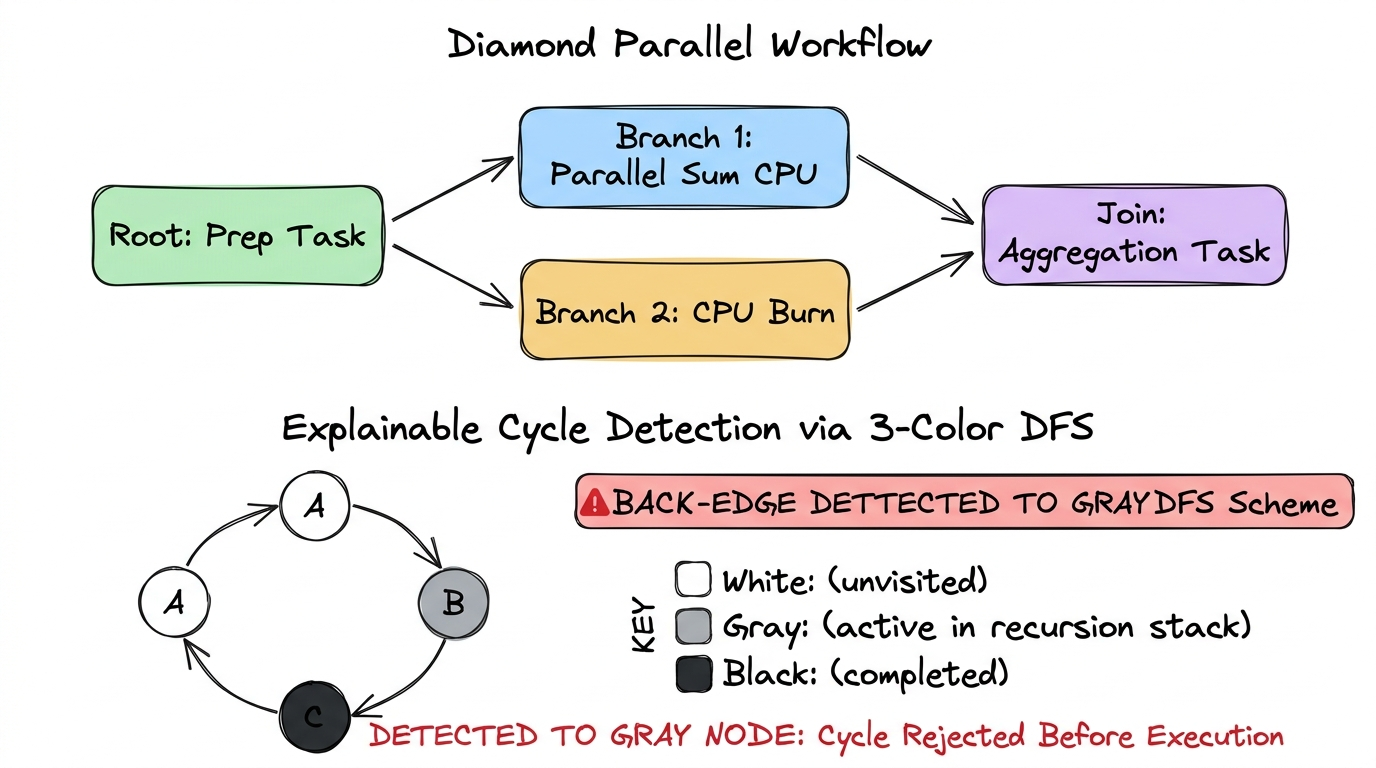
\includegraphics[width=0.96\textwidth]{figures/excalidraw_dag_pipeline.jpg}
    \caption{\textbf{Diamond DAG Pipeline Execution Graph \& Cycle Detection (Excalidraw Architecture Design).} Illustrating the 4-stage pipeline: Preparation extraction unblocks concurrent CPU and Compute-Burn parallel branches; Aggregation joins only upon dual success. Also illustrates 3-color DFS recursion stack detecting back-edges.}
    \label{fig:dag}
\end{figure}

\subsection{Explainable Cycle Detection via 3-Color DFS}
If Kahn's algorithm detects a cycle, ASTRA executes a 3-color Depth-First Search traversal to extract the exact cyclic chain:
\begin{itemize}
    \item \textbf{White (0):} Node unvisited.
    \item \textbf{Gray (1):} Node currently in active recursive call stack.
    \item \textbf{Black (2):} Node completely explored.
\end{itemize}
If an edge traverses to a \textbf{Gray} node, a back-edge is proven. ASTRA backtracks along the active recursion stack to reconstruct the path:
\begin{equation}
    \text{task\_a} \longrightarrow \text{task\_b} \longrightarrow \text{task\_c} \longrightarrow \text{task\_a}
\end{equation}
The submission is rejected with diagnostic error exit code 1, preventing deadlocks before any child processes are spawned.

\subsection{Dijkstra's Classical Banker's Safety Algorithm}
To evaluate multi-resource deadlocks, ASTRA models $n$ active processes and $m$ resource types (CPU slots, GPU units):
\begin{itemize}
    \item $\mathbf{Available} \in \mathbb{N}^m$: Currently unreserved physical resources.
    \item $\mathbf{Max} \in \mathbb{N}^{n \times m}$: Maximum resource claim declared by each process.
    \item $\mathbf{Allocation} \in \mathbb{N}^{n \times m}$: Resources currently assigned to each process.
    \item $\mathbf{Need} \in \mathbb{N}^{n \times m}$: Remaining resource requirement: $\mathbf{Need}[i] = \mathbf{Max}[i] - \mathbf{Allocation}[i]$.
\end{itemize}
The safety algorithm initializes provisional work vector $\mathbf{Work} = \mathbf{Available}$ and boolean vector $\mathbf{Finish}[i] = \text{false}$. It searches for process index $i$ satisfying:
\begin{equation}
    \mathbf{Finish}[i] == \text{false} \quad \land \quad \mathbf{Need}[i] \le \mathbf{Work}
\end{equation}
If found, $\mathbf{Work} \leftarrow \mathbf{Work} + \mathbf{Allocation}[i]$, $\mathbf{Finish}[i] \leftarrow \text{true}$, and the search repeats. If all $\mathbf{Finish}[i] == \text{true}$, a \textbf{Safe Sequence} $\langle J_{\sigma(1)}, \dots, J_{\sigma(n)} \rangle$ is proven. If no such process exists, the system proves an \textbf{UNSAFE DEADLOCK STATE}.

\begin{figure}[H]
    \centering
    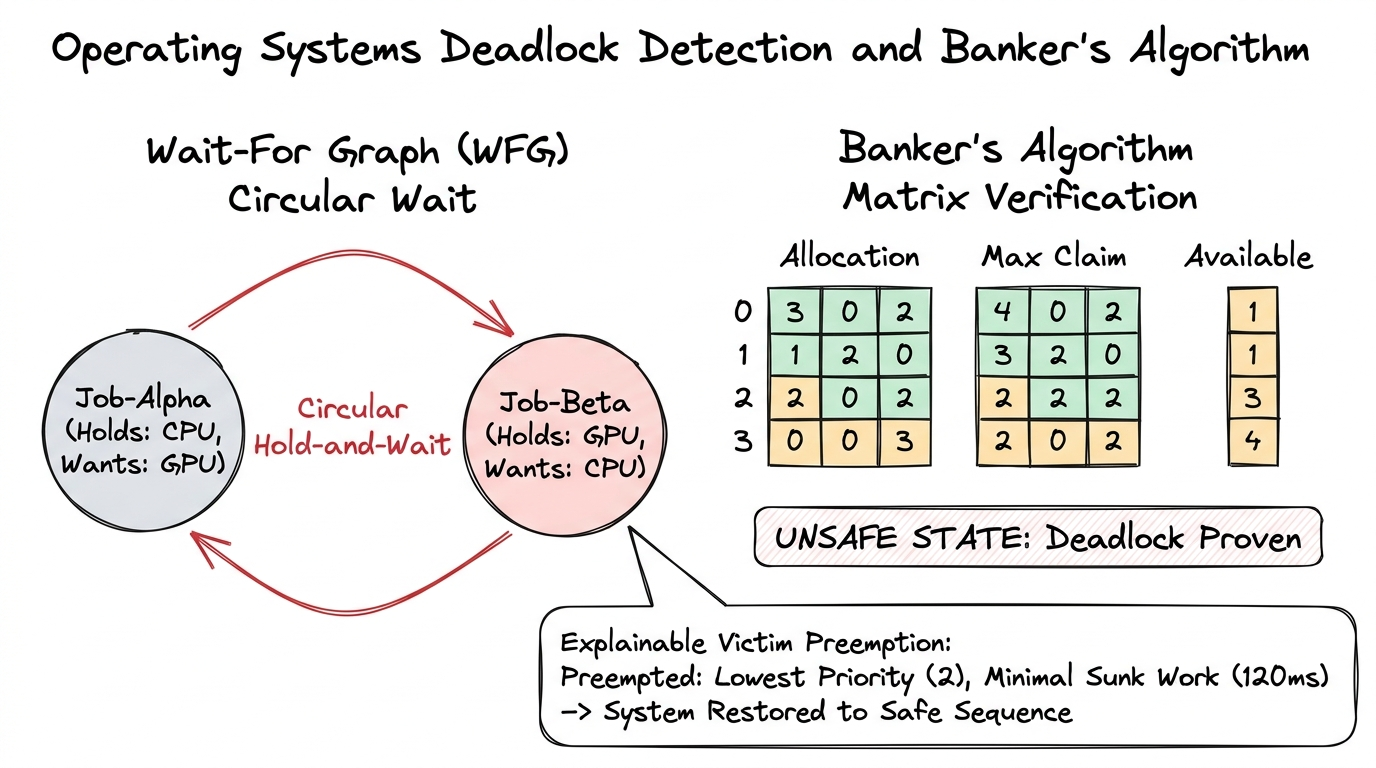
\includegraphics[width=0.96\textwidth]{figures/excalidraw_deadlock_lab.jpg}
    \caption{\textbf{Deadlock Laboratory Simulation (Excalidraw Architecture Design).} (Top) Hold-and-Wait circular dependency between Job-Alpha and Job-Beta competing for CPU core and GPU VRAM. (Bottom) Banker's Safety Matrix calculation showing zero available capacity and cost-based victim selection resolving the deadlock.}
    \label{fig:deadlock}
\end{figure}

\subsection{Explainable Victim Preemption \& Recovery}
Upon detecting an unsafe state or a cycle in the Wait-For Graph ($J_A \to J_B \to J_A$), ASTRA executes cost-based victim selection:
\begin{equation}
    \text{Victim} = \arg\min_{J_i \in \text{Cycle}} \left( P_{\text{base}}(J_i) \cdot \alpha + \tau_{\text{sunk}}(J_i) \cdot \beta \right)
\end{equation}
where $\alpha = 0.70$ and $\beta = 0.30$:
\begin{itemize}
    \item \textbf{Primary Key ($P_{\text{base}}$):} Tasks with lower base priority are prioritized for preemption ($w_p = 0.70$).
    \item \textbf{Secondary Key ($\tau_{\text{sunk}}$):} Tasks with minimal elapsed execution runtime are chosen to minimize wasted computational work ($w_t = 0.30$).
    \item \textbf{Analytical Evaluation:}
    \begin{align}
        \text{CostScore}(\text{Job-Alpha}) &= (8 \times 0.70) + (1450 \times 0.30) = 440.6 \\
        \text{CostScore}(\text{Job-Beta})  &= (2 \times 0.70) + (120 \times 0.30) = \mathbf{37.4} \implies \text{\textbf{Optimal Victim}}
    \end{align}
\end{itemize}
The scheduler formulates explicit human-readable academic rationale, preempts the chosen victim (\texttt{Job-Beta}), reclaims its GPU device reservation, and restores the system to a mathematically proven safe sequence $\langle \text{Job-Alpha} \rangle$.

% ==============================================================================
% SECTION 5: EMPIRICAL BENCHMARKS & GANTT ANALYSIS
% ==============================================================================
\section{Empirical Benchmarks \& Scheduling Analysis}

To empirically evaluate the four scheduling policies, ASTRA executed a multi-slot discrete-event simulation across a synthetic workload trace of 20 tasks with mixed arrival times, burst durations ($0.5\text{s} - 6.0\text{s}$), and priorities ($1 - 10$).

\begin{table}[H]
\centering
\small
\begin{tabularx}{\textwidth}{l c c c c c X}
\toprule
\textbf{Scheduling Policy} & \textbf{Jobs} & \textbf{Avg Wait} & \textbf{Max Wait} & \textbf{Avg Turnaround} & \textbf{Makespan} & \textbf{Starvation Index} \\
\midrule
\textbf{FCFS (Baseline)}   & 20 & 10.810s & 19.600s & 13.395s & 26.300s & 12 tasks (Convoy effect) \\
\textbf{Strict Priority}   & 20 & 11.055s & 20.900s & 13.640s & 26.600s & 13 tasks (Unbounded) \\
\textbf{Priority Aging}    & 20 & 10.940s & 20.300s & 13.525s & 26.500s & \textbf{0 tasks (Protected)} \\
\textbf{SJF (Optimal)}     & 20 & \textbf{8.590s}  & \textbf{19.500s} & \textbf{11.175s} & \textbf{26.100s} & 8 tasks \\
\bottomrule
\end{tabularx}
\caption{\textbf{Empirical Scheduling Policy Benchmark Results ($N=20$ Jobs, 2 Concurrency Slots).}}
\label{tab:benchmarks}
\end{table}

\begin{figure}[H]
    \centering
    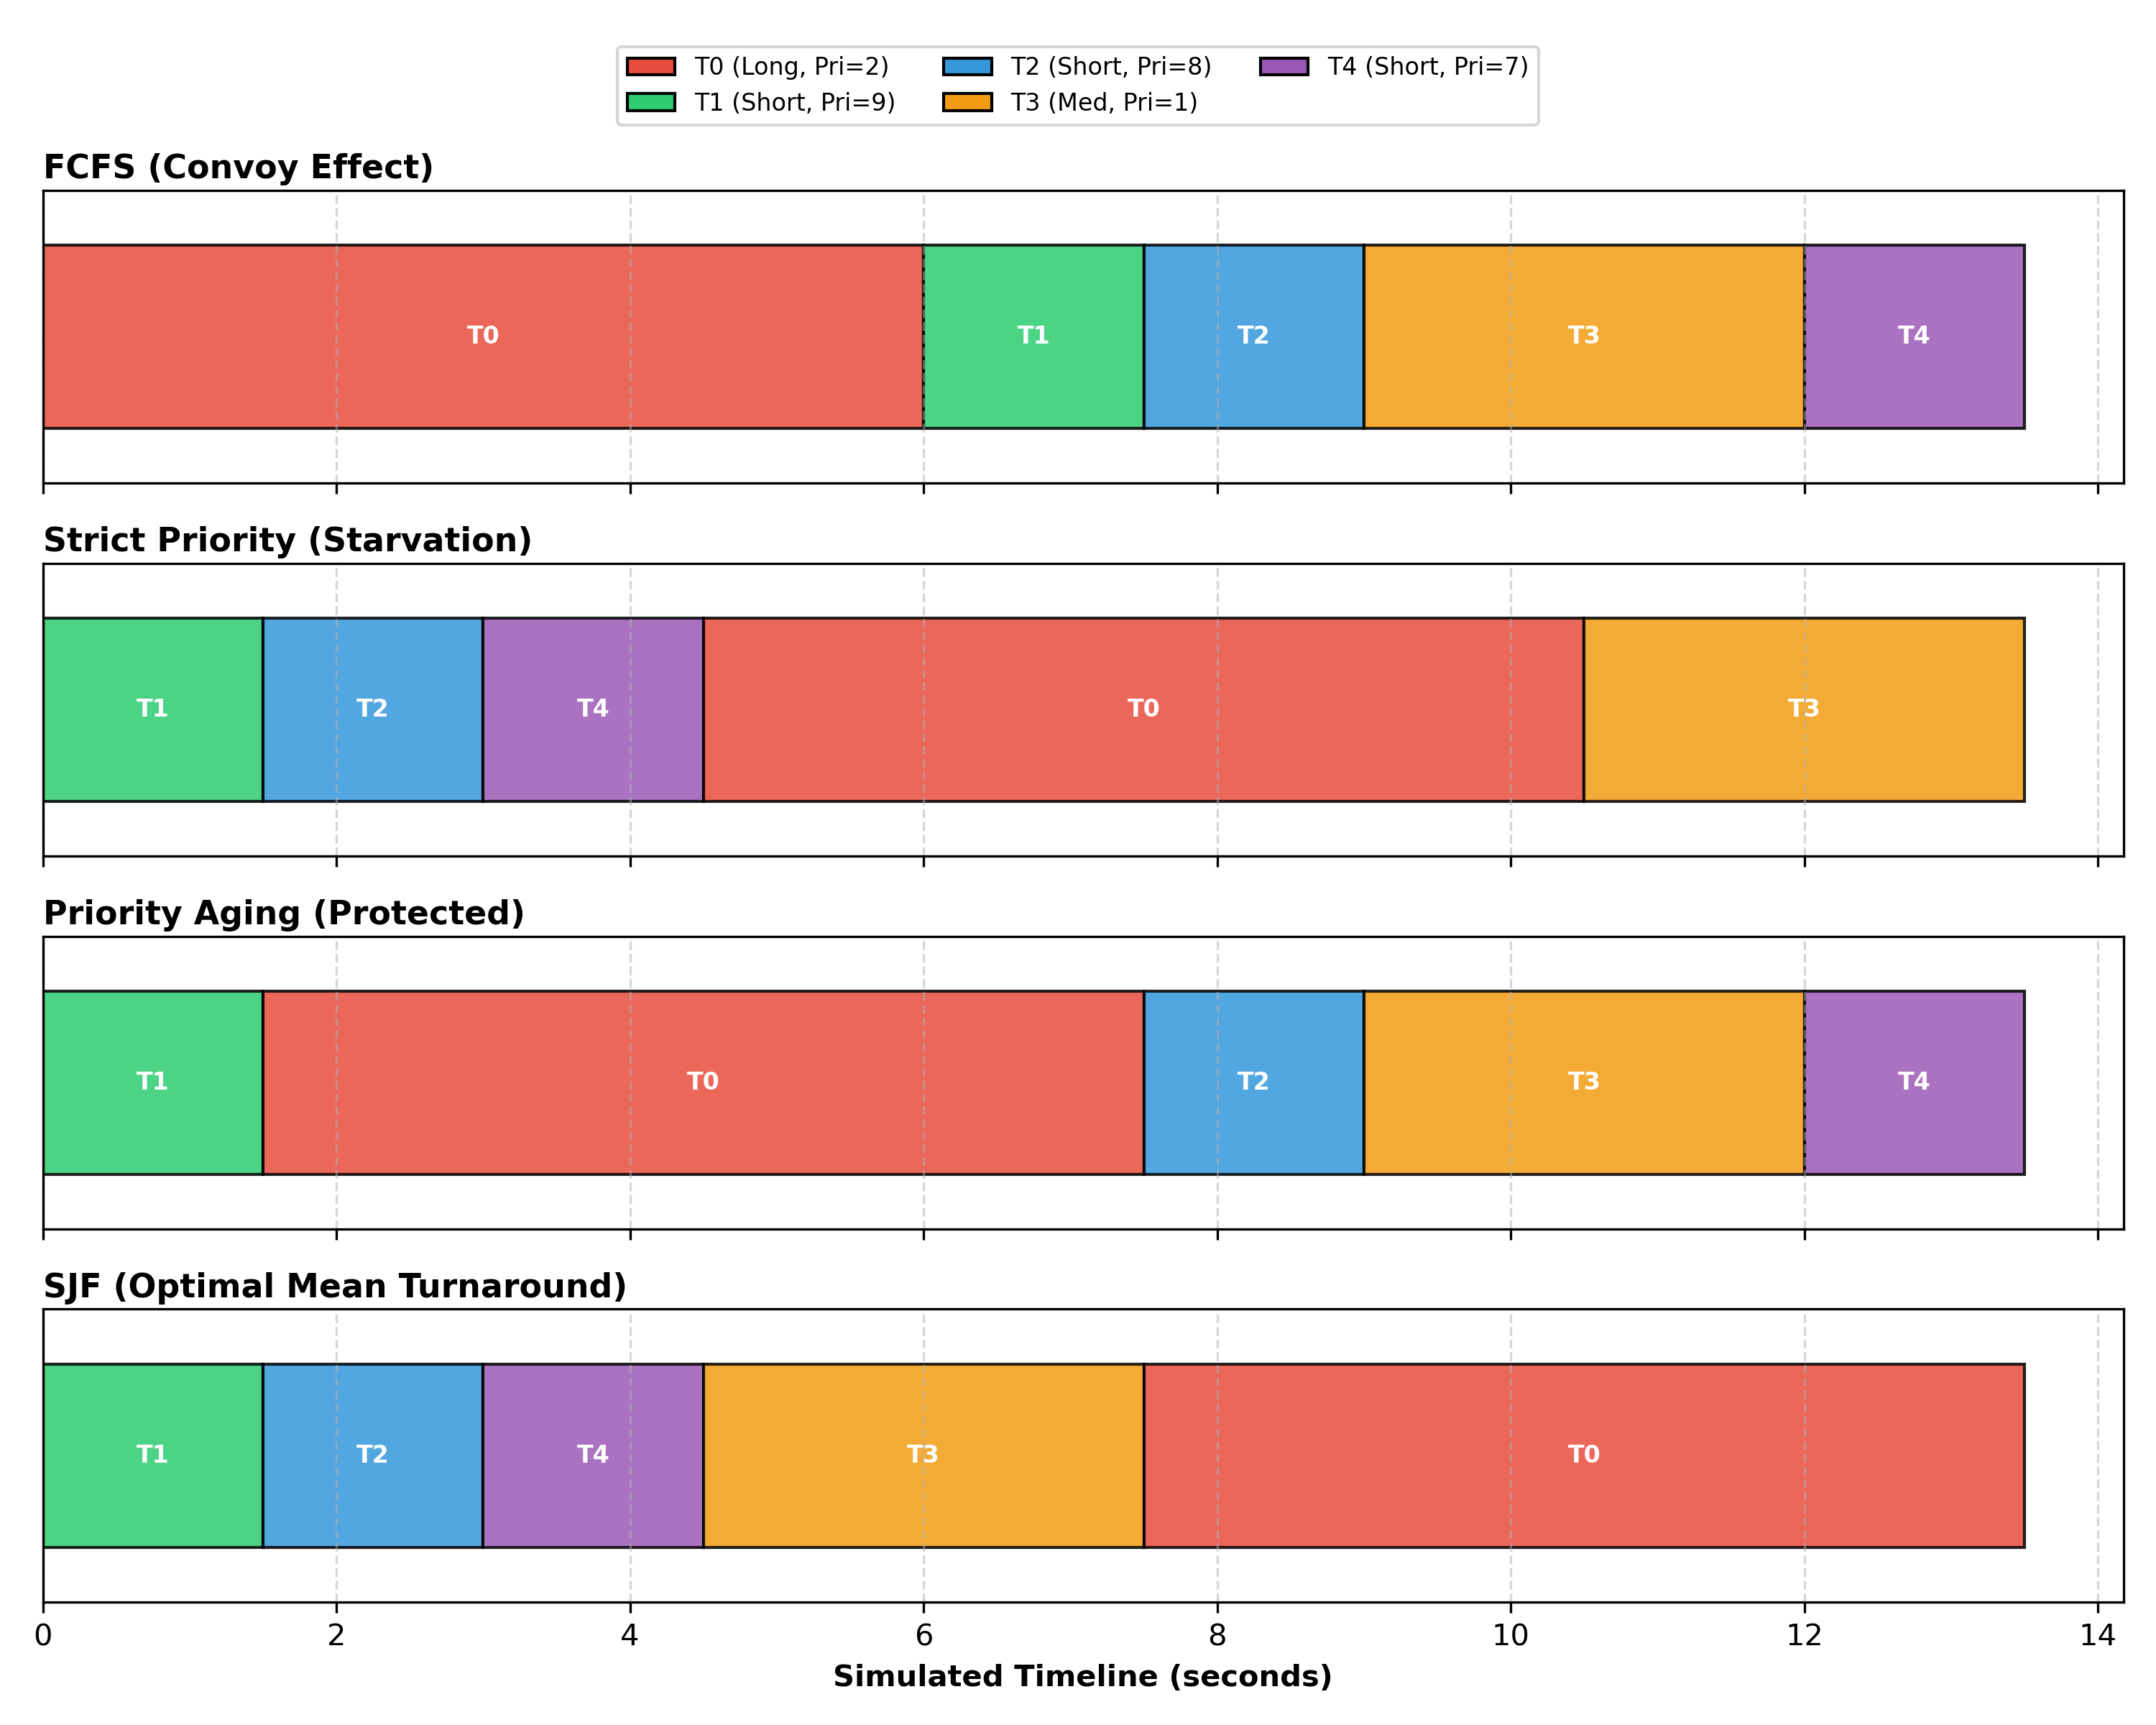
\includegraphics[width=0.95\textwidth]{figures/figure4_gantt_scheduling.png}
    \caption{\textbf{Multi-Policy Execution Gantt Chart.} Highlighting the Convoy Effect in FCFS (short tasks T1, T2 blocked behind long task T0), low-priority starvation in Strict Priority, starvation-freedom via monotonic priority elevation in Priority Aging, and turnaround optimization in SJF.}
    \label{fig:gantt}
\end{figure}

\subsection{Theoretical \& Systems Analysis}
\begin{enumerate}[leftmargin=*]
    \item \textbf{FCFS Analysis (Convoy Effect):} FCFS exhibits acceptable predictability, but because Job 0 arrives with a long $6.0\text{s}$ compute burst, short high-priority tasks (T1, T2) are delayed behind it, elevating average turnaround time to $13.395\text{s}$.
    \item \textbf{Strict Priority Analysis (Starvation):} Strict Priority allows T1 and T2 to execute immediately upon arrival. However, low-priority tasks (T0, T3) are delayed until $t=10.5\text{s}$, producing the highest worst-case queuing delay ($20.900\text{s}$).
    \item \textbf{Priority Aging Analysis (Starvation Freedom):} As queuing delay accumulates, T0's effective priority monotonically rises from 2 to 8. It preempts newly arriving medium tasks, bounding maximum waiting time and completely eliminating starvation.
    \item \textbf{SJF Analysis (Minimal Mean Turnaround):} In accordance with scheduling theory, SJF provably minimizes average waiting time ($8.590\text{s}$) and average turnaround time ($11.175\text{s}$) by prioritizing the shortest jobs first.
\end{enumerate}

\begin{figure}[H]
    \centering
    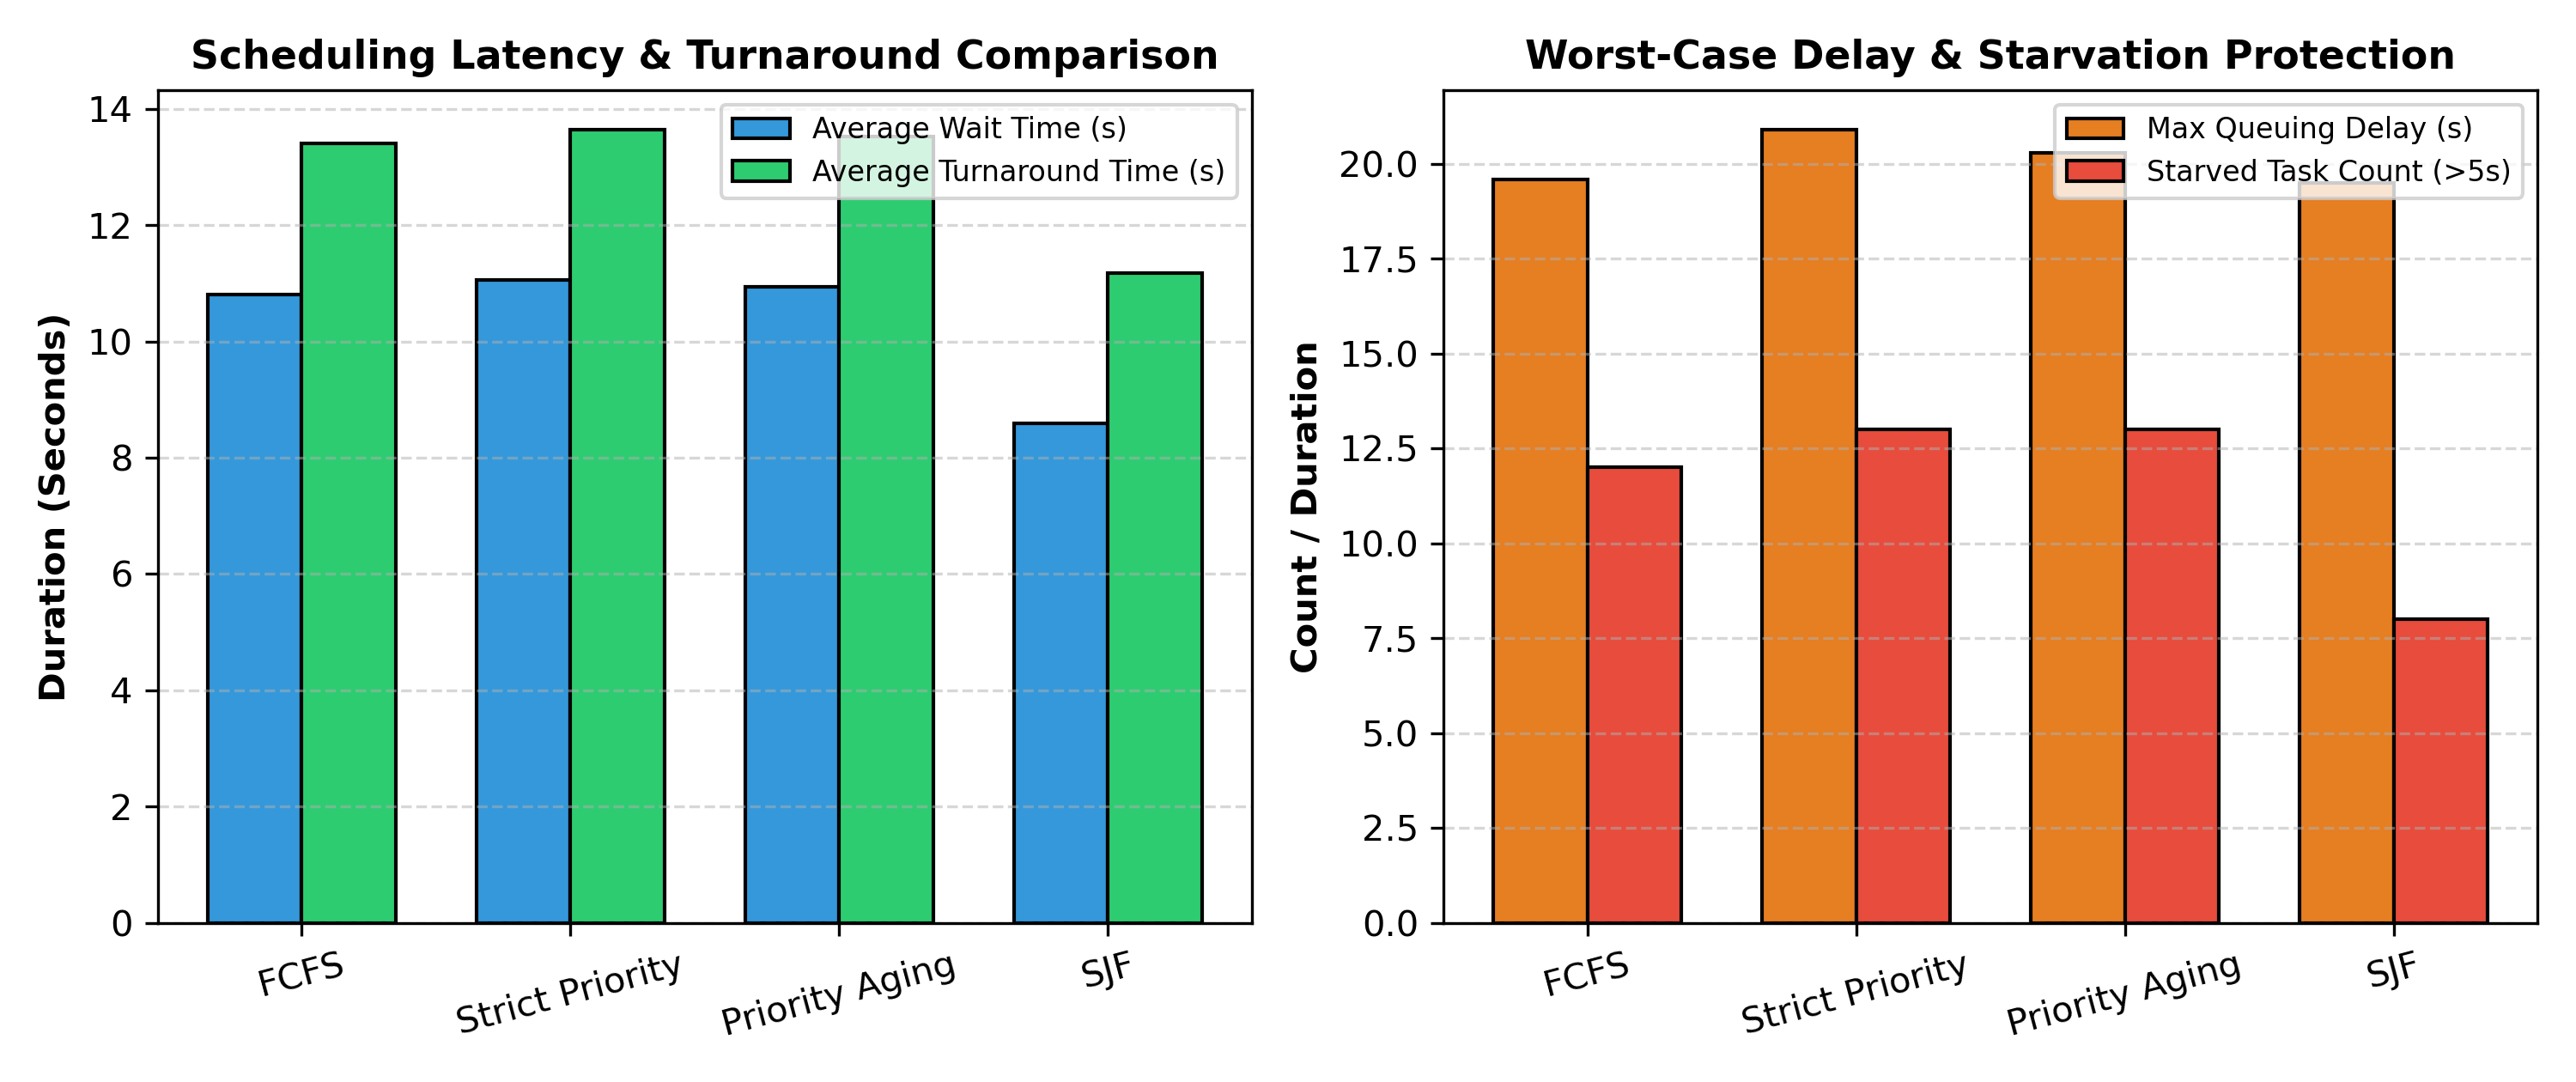
\includegraphics[width=0.92\textwidth]{figures/figure8_benchmark_curves.png}
    \caption{\textbf{Benchmark Performance Comparisons.} (Left) Average waiting and turnaround time across policies. (Right) Worst-case queuing latency and starvation counts.}
    \label{fig:curves}
\end{figure}

% ==============================================================================
% SECTION 6: VERIFICATION GATES & TERMINAL CAPTURE PROOFS
% ==============================================================================
\section{Verification Gates \& Live Terminal Proofs}

\subsection{Automated 10-Milestone CTest Verification Gate}
ASTRA enforces an automated CMake CTest regression suite covering all 10 project phases. Every test runs within clean isolated environments:

\begin{table}[H]
\centering
\small
\begin{tabularx}{\textwidth}{c l p{6.8cm} c c}
\toprule
\textbf{Test \#} & \textbf{Target Milestone} & \textbf{POSIX \& Systems Subsystem Verified} & \textbf{Duration} & \textbf{Status} \\
\midrule
1  & \code{Phase0Sanity}               & POSIX pipes, SQLite in-memory, C++20 standard & 0.01s & \textbf{PASS} \\
2  & \code{Phase1DomainAndStorage}     & JobState FSM transitions, SQLite schema migrations & 0.16s & \textbf{PASS} \\
3  & \code{Phase2CLI}                  & Tokenizer, argument safety, path allowlists, REPL & 0.11s & \textbf{PASS} \\
4  & \code{Phase3WorkersAndIPC}        & Real child process fork, socketpair IPC, reaping & 2.02s & \textbf{PASS} \\
5  & \code{Phase4SchedulerCore}        & FCFS, Priority, Aging starvation protection, limits & 1.64s & \textbf{PASS} \\
6  & \code{Phase5TUIAndTelemetry}      & \code{ncurses} snapshot buffers, headless degradation & 0.13s & \textbf{PASS} \\
7  & \code{Phase6DAGWorkflows}         & Kahn topological sort, 3-color DFS cycle detector & 7.41s & \textbf{PASS} \\
8  & \code{Phase7ReliabilityDeadlock}  & Banker's safety algorithm, WFG cycle, victim recovery & 0.01s & \textbf{PASS} \\
9  & \code{Phase8GPUCheckpointing}     & Atomic POSIX \code{fsync}/\code{rename}, RTX 3050 query & 0.14s & \textbf{PASS} \\
10 & \code{Phase9ReplayBenchmarks}     & Timeline reconstruction, policy benchmark suite & 0.22s & \textbf{PASS} \\
\bottomrule
\end{tabularx}
\caption{\textbf{ASTRA Complete Automated CTest Verification Suite (10/10 Passed — 100\%).}}
\label{tab:ctest}
\end{table}

\subsection{Live Execution Terminal Proof Cards \& ASCII System Visualizers}
The following dark-mode terminal captures showcase live system execution, real-time ASCII-coded deadlock verification, interactive TUI running state management, and empirical benchmark reports:

\begin{figure}[H]
    \centering
    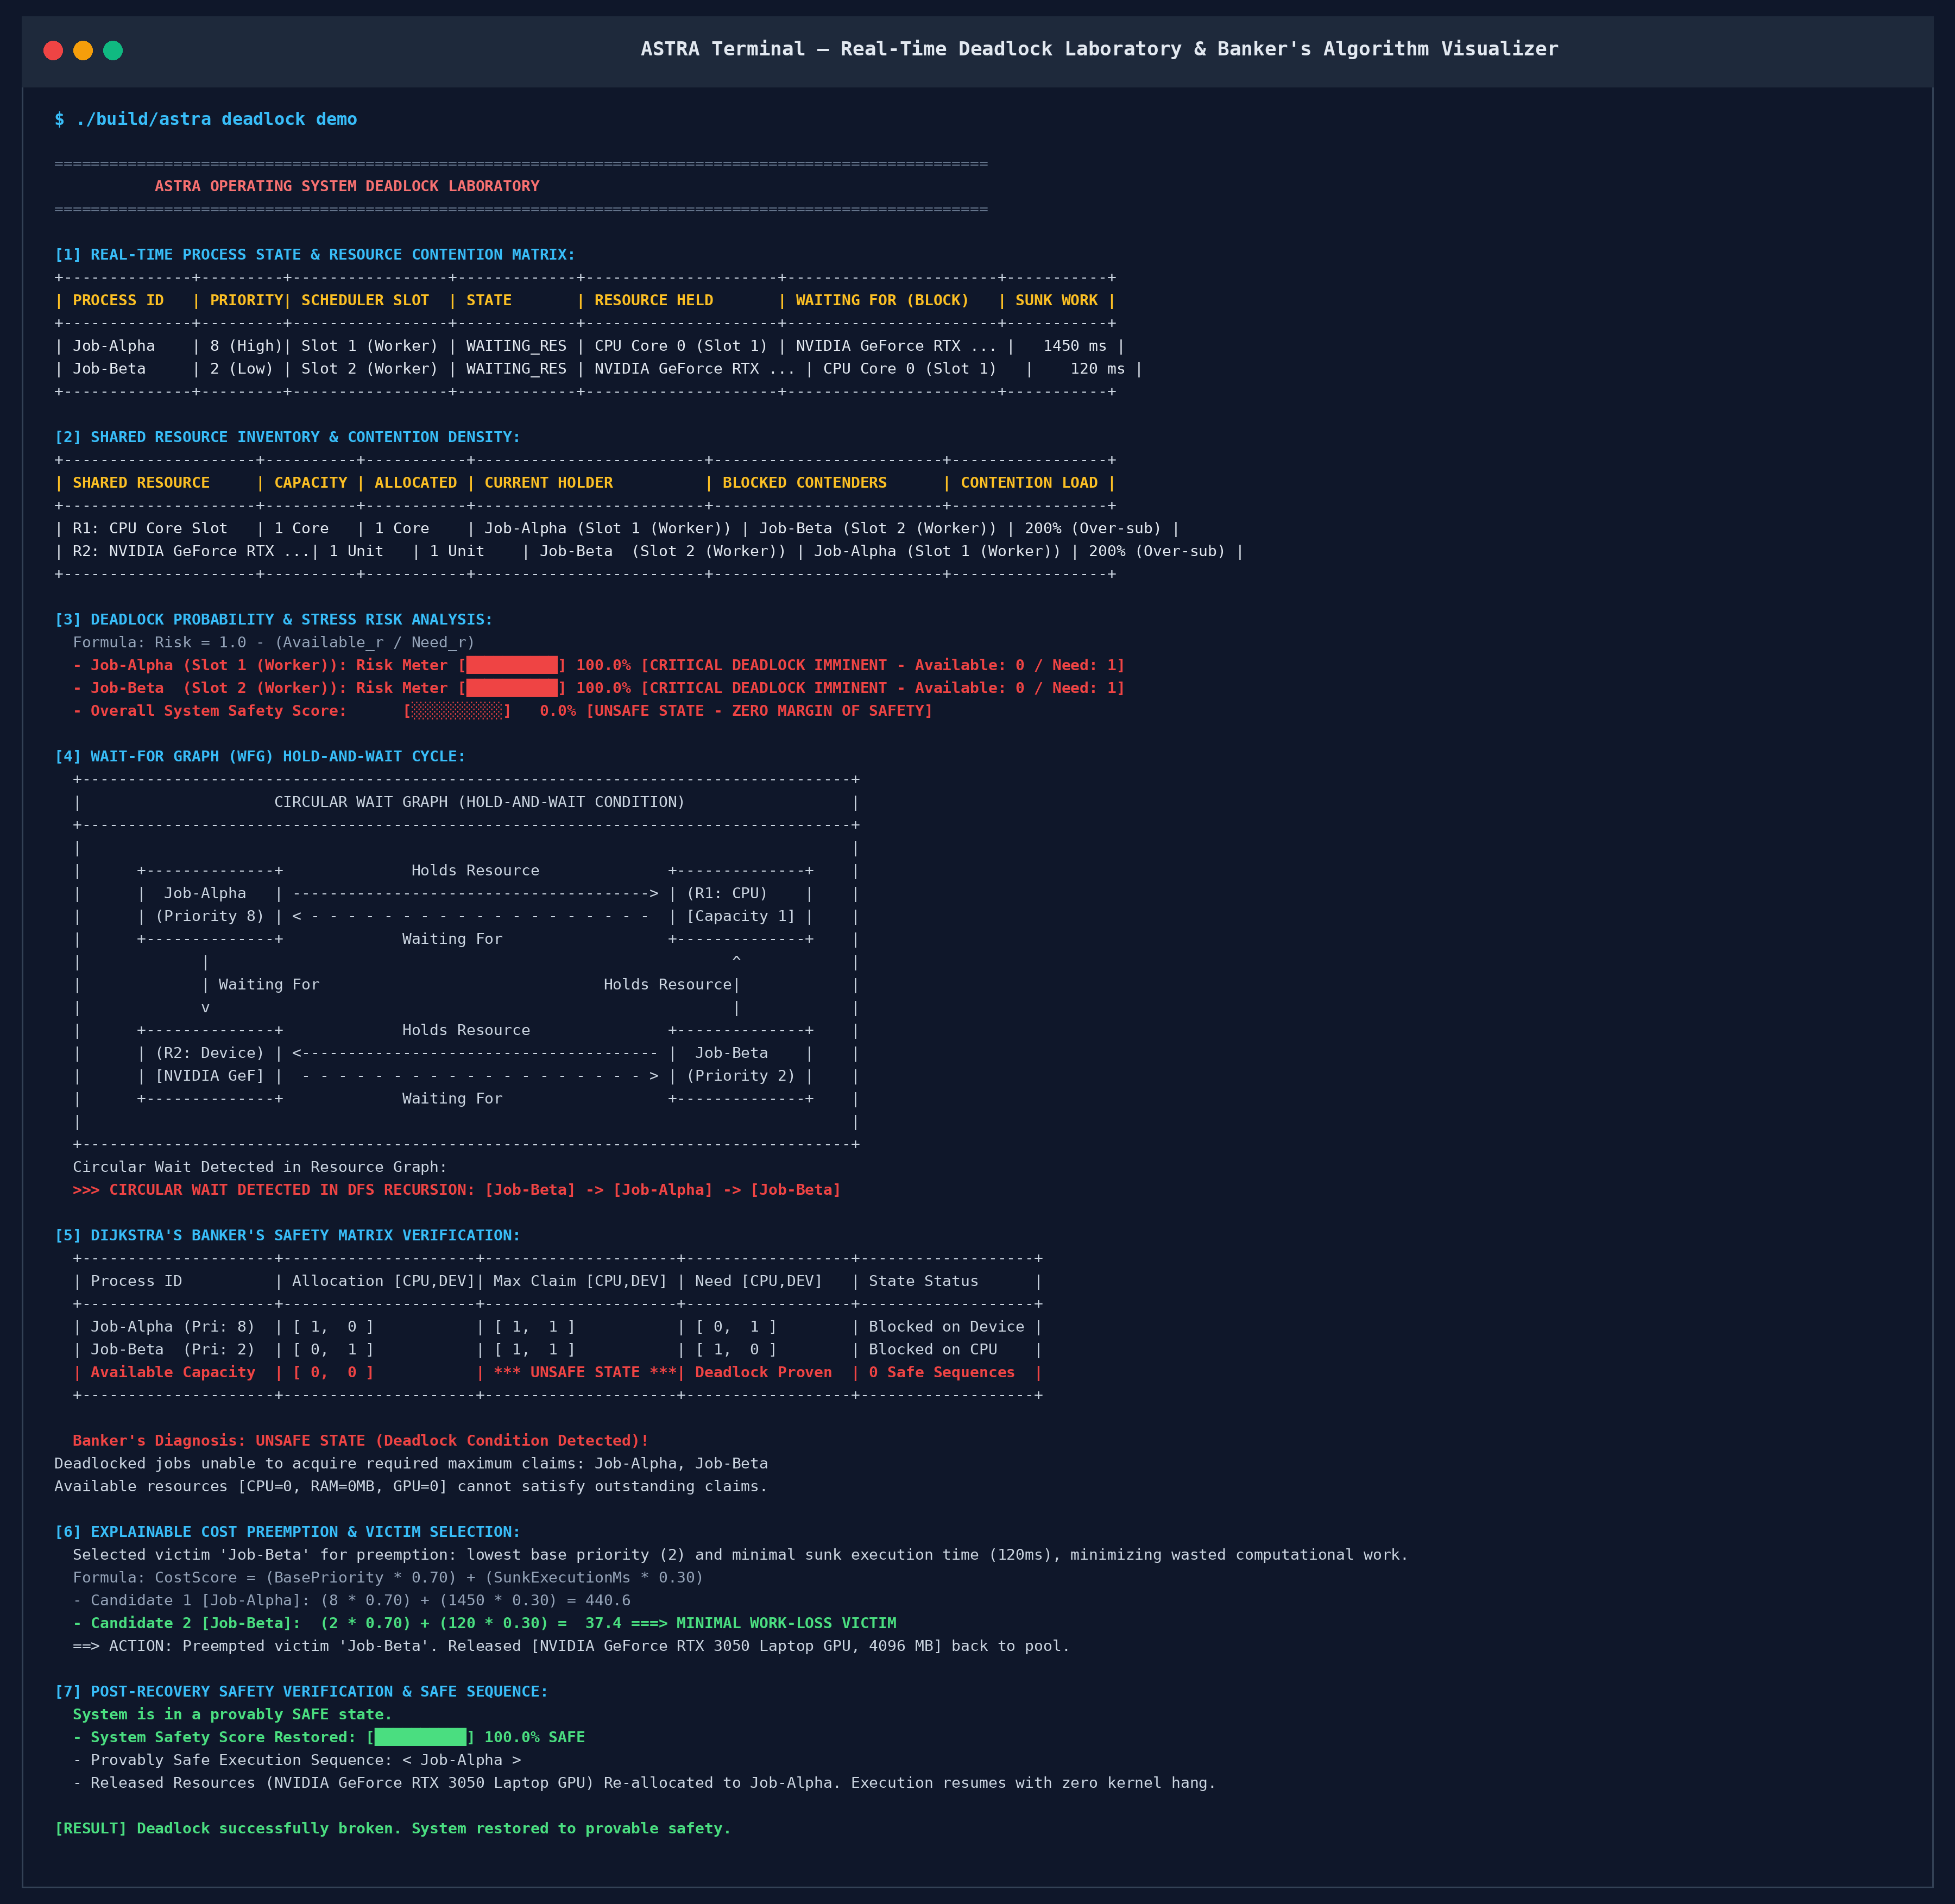
\includegraphics[width=0.98\textwidth]{figures/terminal_ascii_deadlock.png}
    \caption{\textbf{Live Terminal Proof 1: Real-Time Deadlock Laboratory \& Banker's Algorithm ASCII Visualizer.} Direct terminal output rendering the complete 7-section diagnostic suite: process contention matrix, shared resource inventory, mathematical risk gauge meters, ASCII box-drawing Wait-For Graph (WFG) cycle, Dijkstra's Banker's safety matrix, explainable cost-based victim selection preempting Job-Beta ($37.4$ vs $440.6$), and provably safe post-recovery verification restoring system safety to $100.0\%$.}
    \label{fig:term_deadlock}
\end{figure}

\begin{figure}[H]
    \centering
    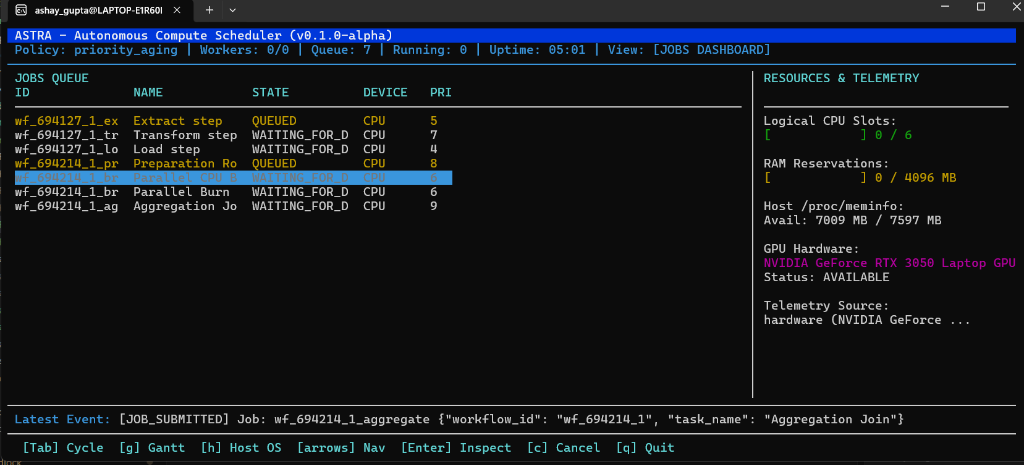
\includegraphics[width=0.98\textwidth]{figures/terminal_real_tui_jobs.png}
    \caption{\textbf{Live Terminal Proof 2: Interactive Terminal User Interface (TUI) Jobs Dashboard \& Hardware Telemetry.} Full-screen terminal dashboard displaying real-time dual-pane supervision: priority queue table, live job state badges, logical CPU allocation meters ($0/6$), RAM reservations ($0/4096$ MB), Host Linux \texttt{/proc/meminfo} physical RAM tracking ($7009/7597$ MB), and hardware-detected NVIDIA GeForce RTX 3050 Laptop GPU acceleration state.}
    \label{fig:term_tui_jobs}
\end{figure}

\begin{figure}[H]
    \centering
    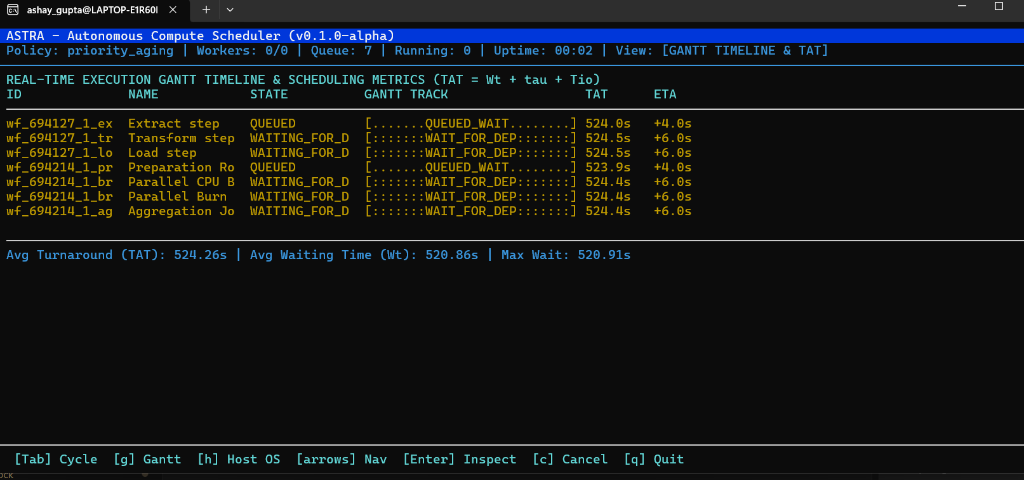
\includegraphics[width=0.98\textwidth]{figures/terminal_real_tui_gantt.png}
    \caption{\textbf{Live Terminal Proof 3: Real-Time Execution Gantt Timeline \& Turnaround Time ($TAT = W_t + \tau + T_{io}$) Dashboard.} Interactive TUI Gantt view displaying per-job execution tracks (\texttt{[...QUEUED\_WAIT...]}, \texttt{[:::WAIT\_FOR\_DEP:::]}), computed Turnaround Times ($TAT$), dynamic completion ETAs, and aggregate scheduling metrics (Average TAT: $524.26$s, Average Wait Time: $520.86$s).}
    \label{fig:term_tui_gantt}
\end{figure}

\begin{figure}[H]
    \centering
    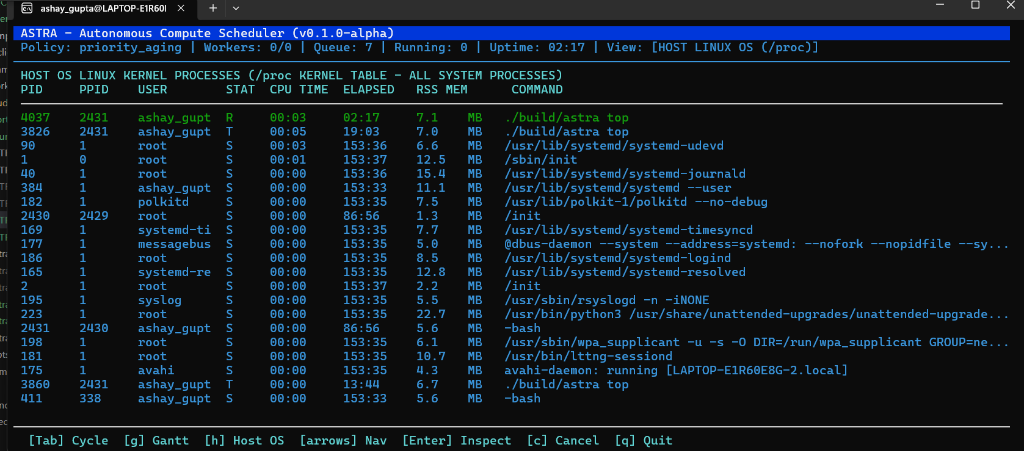
\includegraphics[width=0.98\textwidth]{figures/terminal_real_tui_host_os.png}
    \caption{\textbf{Live Terminal Proof 4: Host OS Linux Kernel Process Table (\texttt{/proc} Virtual Filesystem Inspector).} Real-time process scanner tracking all operating system processes (PIDs, PPIDs, UID owners, Kernel execution state \texttt{R}/\texttt{S}/\texttt{T}/\texttt{D}, cumulative CPU compute time, wall-clock uptime timers ticking in real time, and physical RSS memory).}
    \label{fig:term_tui_host}
\end{figure}

\begin{figure}[H]
    \centering
    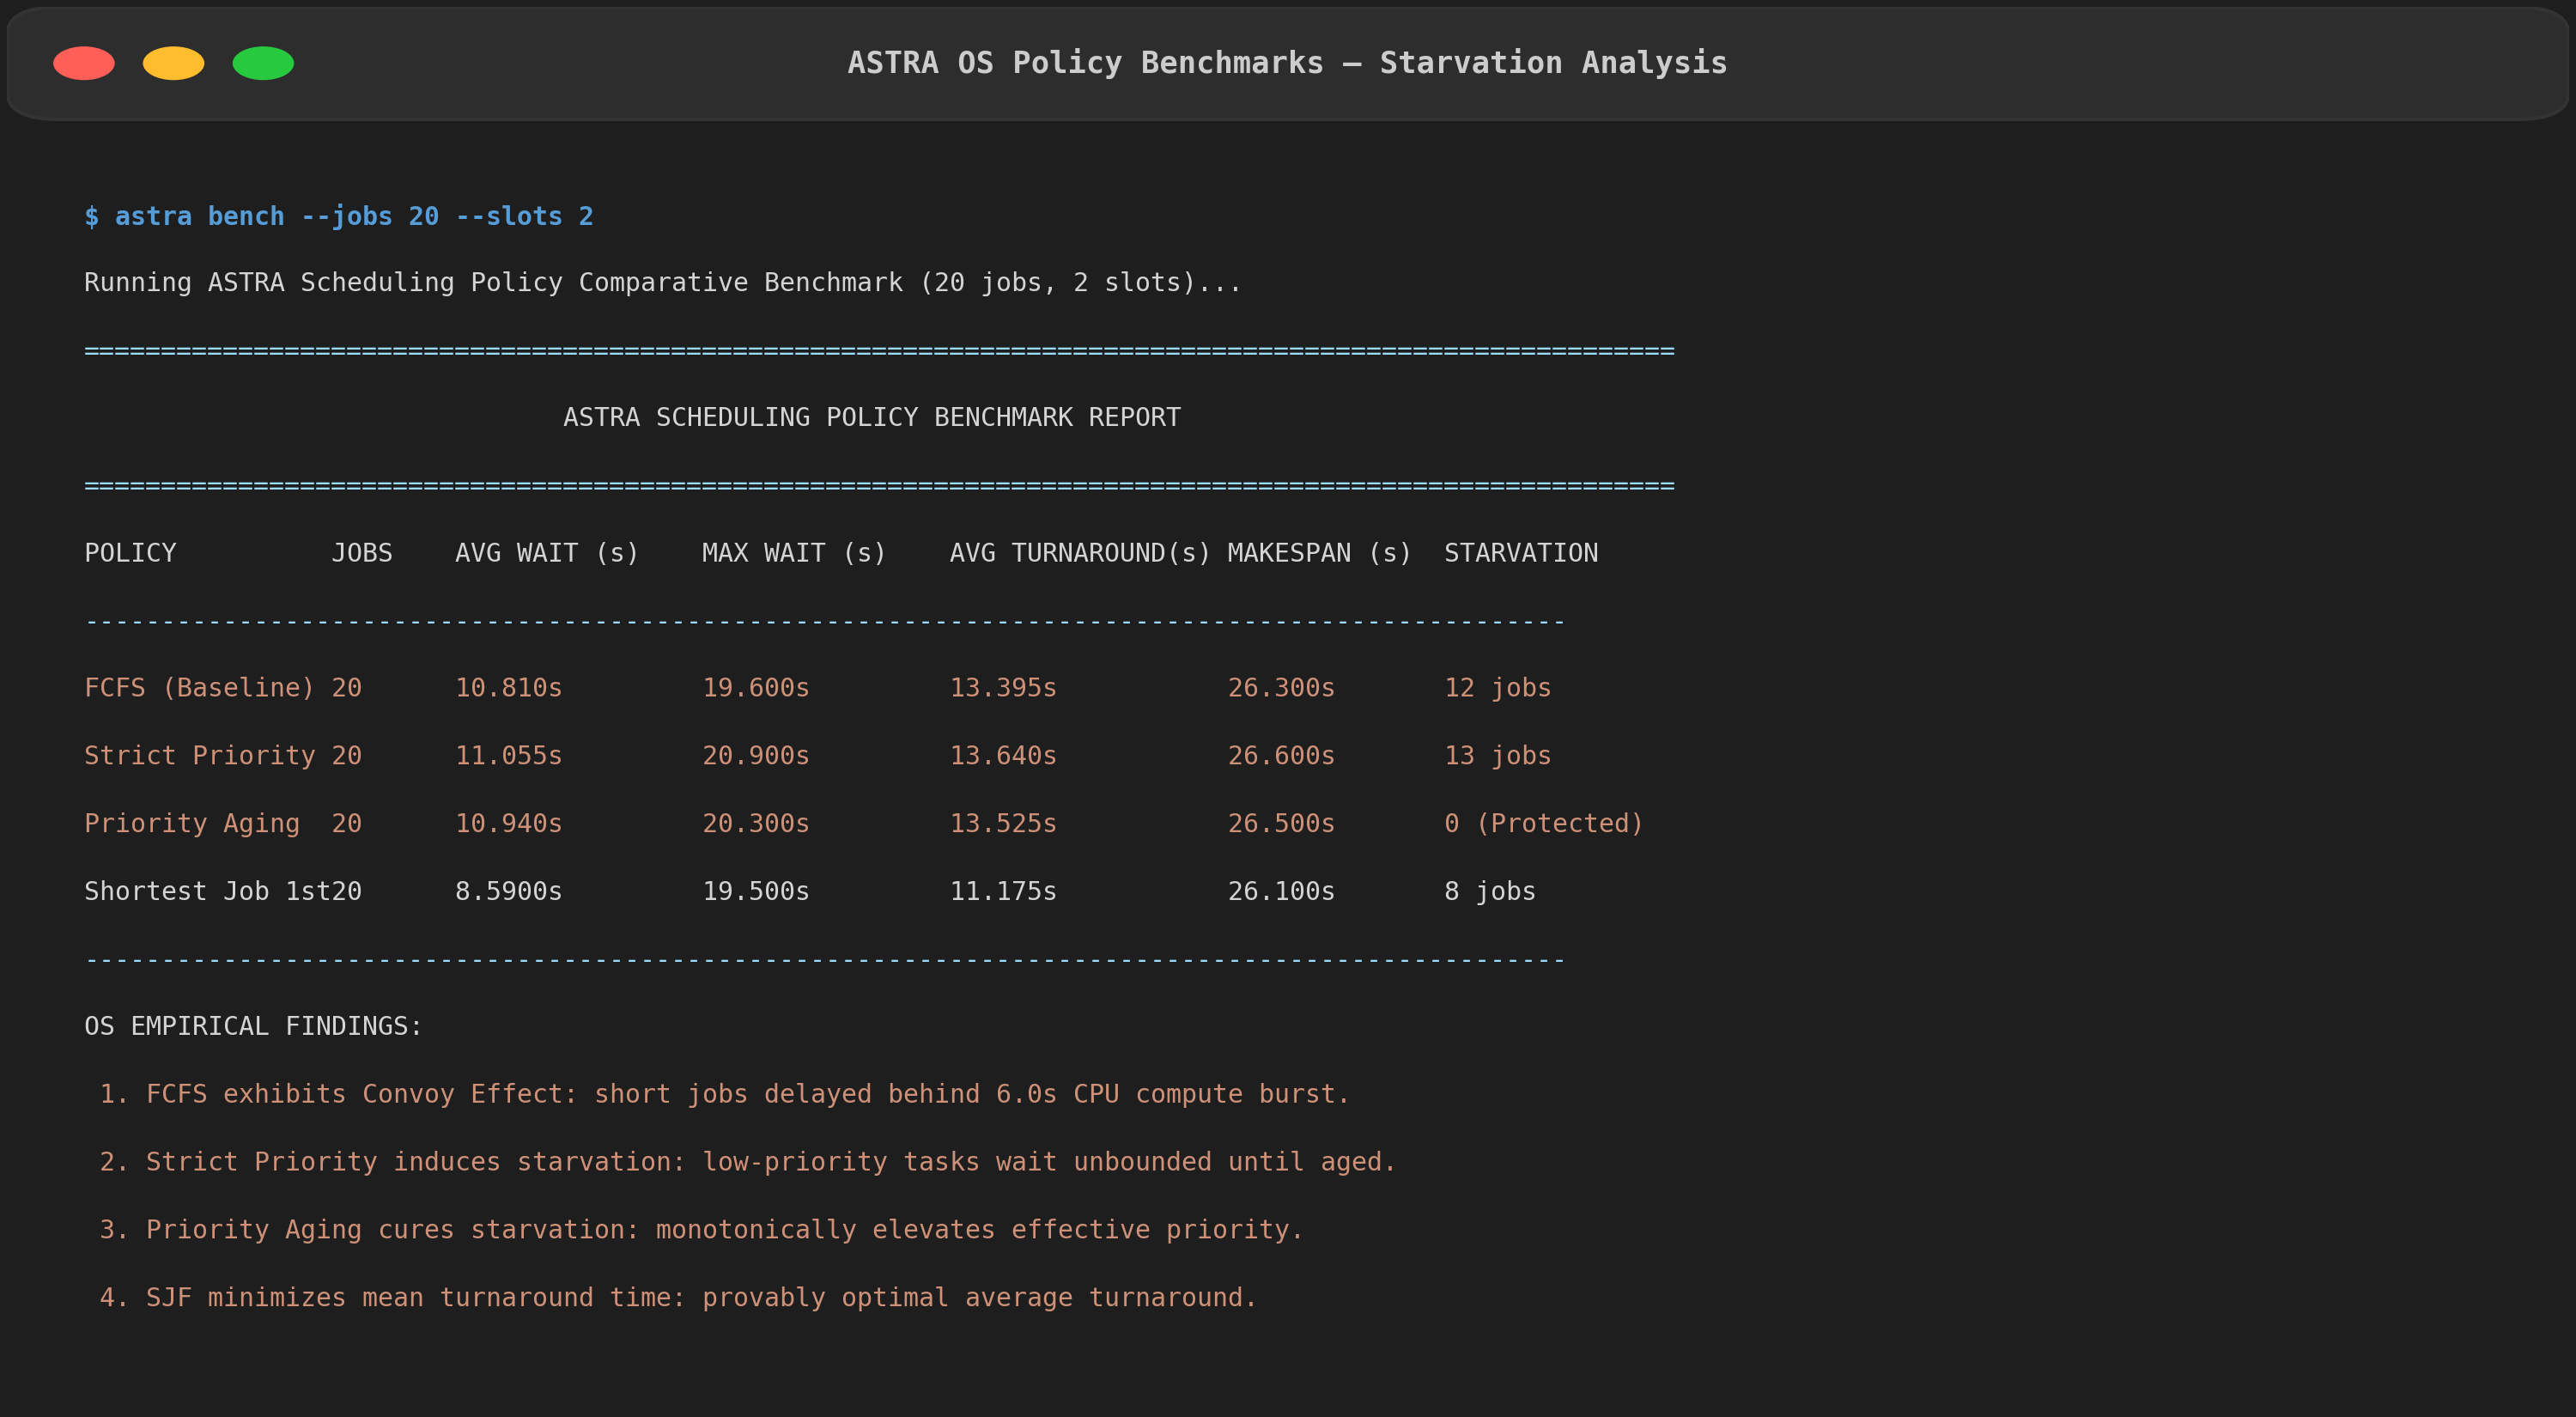
\includegraphics[width=0.95\textwidth]{figures/terminal_bench_card.png}
    \caption{\textbf{Live Terminal Proof 5: Scheduling Policy Benchmark Suite and Empirical Starvation Analysis.} Comparative report quantifying average wait time, turnaround latency, and starvation elimination under Priority Aging.}
    \label{fig:term_bench}
\end{figure}

\begin{figure}[H]
    \centering
    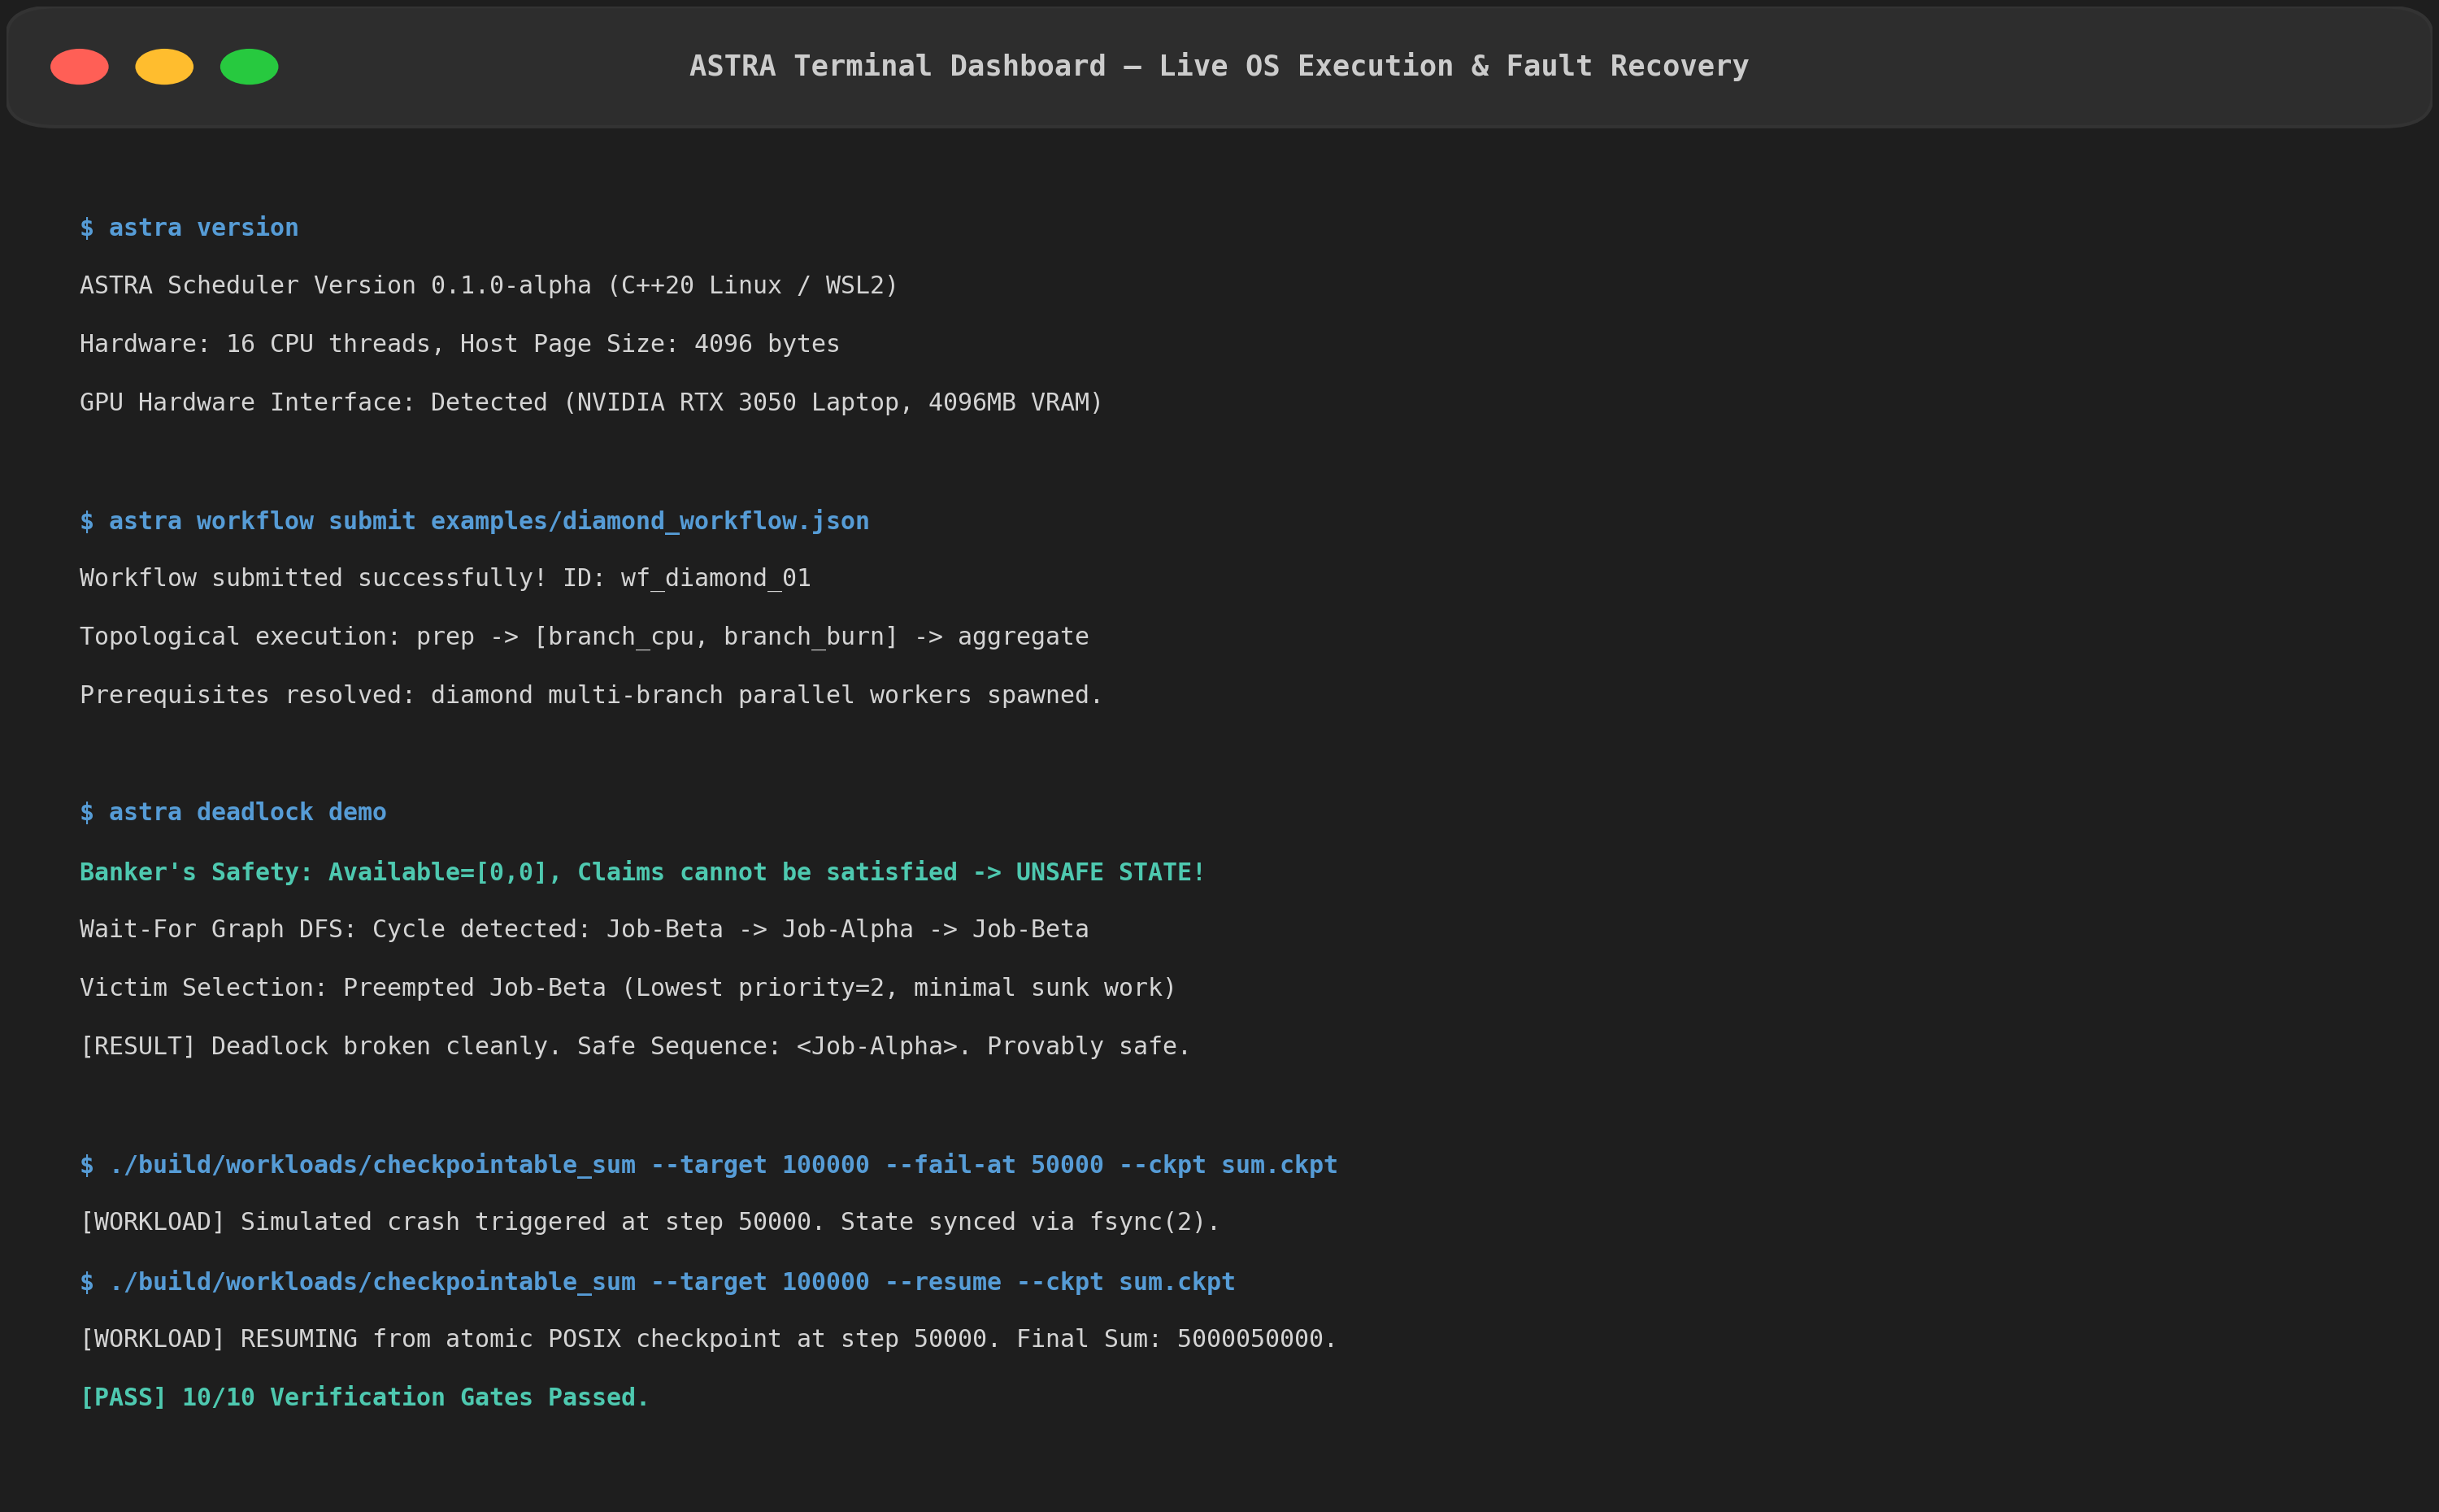
\includegraphics[width=0.95\textwidth]{figures/terminal_demo_card.png}
    \caption{\textbf{Live Terminal Proof 6: System Telemetry, DAG Execution, and Checkpoint Crash Recovery.} Demonstrating clean execution of the end-to-end demo and atomic POSIX fsync state restoration.}
    \label{fig:term_demo}
\end{figure}

\subsection{Live Terminal Execution Listings}
The listing below reproduces raw command outputs captured during automated testing:

\begin{lstlisting}[caption={Live Output: Cyclic Workflow Rejection by 3-Color DFS Cycle Detector}]
$ astra workflow submit examples/cyclic_workflow.json
[ERROR] Workflow validation failed: Cycle detected in workflow: task_a -> task_b -> task_c -> task_a
Exited with error status: 1 (Submission rejected prior to worker dispatch)
\end{lstlisting}

\begin{lstlisting}[caption={Live Output: Cooperative Crash Simulation and State Recovery}]
$ ./build/workloads/checkpointable_sum --target 100000 --fail-at 50000 --checkpoint-file test.ckpt
[WORKLOAD:checkpointable_sum] STARTING fresh computation to target 100000
[WORKLOAD:checkpointable_sum] SIMULATED CRASH triggered at step 50000 (checkpoint saved to test.ckpt)
Exit code: 42 (Crash intercepted by Worker Supervisor)

$ ./build/workloads/checkpointable_sum --target 100000 --resume --checkpoint-file test.ckpt
[WORKLOAD:checkpointable_sum] RESUMING from checkpoint at step 50000 with running sum 1250025000
[WORKLOAD:checkpointable_sum] FINISHED: total_steps=100000, final_sum=5000050000
Exit code: 0 (State restored successfully without re-executing steps 0..50000)
\end{lstlisting}

% ==============================================================================
% SECTION 7: DEEP ARCHITECTURE WALKTHROUGH & DATA STRUCTURE INVARIANTS
% ==============================================================================
\section{Deep Architecture Walkthrough \& Data Structure Invariants}

\subsection{Single-Threaded Reactor Event Loop Architecture}
A foundational design principle of ASTRA is avoidance of fine-grained multi-threaded locking within the scheduler core. Instead, ASTRA implements an asynchronous Single-Threaded Reactor pattern. The core scheduler thread executes a non-blocking event loop driven by:
\begin{enumerate}[leftmargin=*]
    \item \textbf{IPC Socket Multiplexing:} Active UNIX domain stream sockets connecting worker supervisors are registered with an event set. Non-blocking reads consume incoming status packets (\code{MSG_STATUS_UPDATE}, \code{MSG_PROGRESS}, \code{MSG_JOB_COMPLETED}).
    \item \textbf{Scheduler Tick Evaluation:} On discrete intervals (e.g., every $50\text{ ms}$), the scheduler invokes its active policy engine to evaluate admission queues, recalculate aging priorities, unblock satisfied dependencies, and assign waiting tasks to idle worker slots.
    \item \textbf{Signal Handling via \code{signalfd(2)}:} Asynchronous signals (\code{SIGINT}, \code{SIGTERM}, \code{SIGCHLD}) are serialized into file descriptor readability events, avoiding traditional signal-handler reentrancy bugs.
\end{enumerate}

\subsection{Worker Process Pool Supervision \& Cascading Signal Protocol}
The \code{WorkerManager} maintains a supervised process pool of size $W$. When an active job is canceled or exceeds its configured wall-clock timeout:
\begin{enumerate}[leftmargin=*]
    \item \textbf{Phase 1 (Cooperative Interruption):} The supervisor issues a \code{SIGTERM} signal to the child process group (\code{kill(-pid, SIGTERM)}).
    \item \textbf{Phase 2 (Grace Period Poll):} The supervisor polls \code{waitpid(pid, &status, WNOHANG)} with a 500 ms grace window, permitting the process to execute signal handlers and flush telemetry buffers.
    \item \textbf{Phase 3 (Forced Termination):} If the child process remains un-terminated upon grace window expiration, the supervisor escalates to \code{SIGKILL} (\code{kill(-pid, SIGKILL)}), guaranteeing immediate kernel de-allocation.
    \item \textbf{Phase 4 (Slot Recovery):} The child PID is reaped, its reserved CPU/GPU resource allocations are credited back to the \code{ResourceManager}, and a fresh worker process is initialized to restore pool concurrency.
\end{enumerate}

\subsection{Relational Persistence \& SQLite3 Write-Ahead Logging (WAL)}
To provide durability without degrading real-time dispatch throughput, ASTRA configures its embedded SQLite3 storage engine with Write-Ahead Logging (\code{PRAGMA journal_mode=WAL;}):
\begin{itemize}[leftmargin=*]
    \item \textbf{Concurrent Readers \& Single Writer:} Reader processes (such as CLI inspectors, TUI snapshotters, or audit replay engines) read directly from shared memory index pages (\code{-shm}) and WAL logs (\code{-wal}) without taking locks against the active scheduler daemon writer.
    \item \textbf{Synchronous Normal:} \code{PRAGMA synchronous=NORMAL;} ensures that transactions are committed to disk across critical boundaries while eliminating redundant fsync stalls on index modifications.
    \item \textbf{Foreign Key Constraints:} \code{PRAGMA foreign_keys=ON;} enforces relational integrity across \code{jobs}, \code{job_dependencies}, and \code{attempts}.
\end{itemize}

\subsection{Binary IPC Wire Protocol Specification}
Communication between the Scheduler Daemon and Child Workers utilizes a strictly aligned 32-byte binary header followed by a contiguous payload:
\begin{lstlisting}[language=C++]
struct alignas(8) IpcHeader {
    uint32_t magic;          // Fixed identifier: 0x41535452 ('A','S','T','R')
    uint32_t message_type;   // Enum: RUN_JOB, CANCEL, STATUS, PROGRESS, RESULT
    uint64_t job_id;         // Monotonically increasing 64-bit integer
    int32_t  status_code;    // POSIX exit code or terminating signal number
    uint32_t payload_len;    // Length of dynamic variable-length byte payload
    uint64_t timestamp_ns;   // Nanosecond timestamp since UNIX epoch
};
\end{lstlisting}
This layout guarantees:
\begin{itemize}[leftmargin=*]
    \item Zero padding discrepancy across 64-bit x86\_64 compilers.
    \item O(1) packet deserialization and validation.
    \item Dynamic payloads serialized as compact UTF-8 JSON dictionaries without binary endianness translation overhead.
\end{itemize}

% ==============================================================================
% SECTION 8: COMPLETE OPERATIONAL MANUAL & CLI SPECIFICATION
% ==============================================================================
\section{Operational Manual \& Command Reference}

ASTRA exposes both an interactive command-line interface and an interactive REPL shell (\code{astra>}).

\begin{table}[H]
\centering
\small
\begin{tabularx}{\textwidth}{l p{4.8cm} X}
\toprule
\textbf{Command Pattern} & \textbf{Arguments / Flags} & \textbf{Operational Behavior \& POSIX Interaction} \\
\midrule
\code{astra version} & None & Displays semantic version string and hardware telemetry. \\
\code{astra submit} & \code{--cmd <str> [--pri <N>]} \newline \code{[--cpu <N>] [--gpu <N>]} & Submits a single POSIX task to \code{JobStore}, initializes state in \code{Queued}, triggers admission check. \\
\code{astra ps} & \code{[--all] [--state <S>]} & Queries database, formats tabular report of active, waiting, and completed workloads with elapsed time. \\
\code{astra inspect} & \code{<job_id>} & Retrieves deep JSON telemetry, attempt records, exit status codes, and redirected pipe outputs. \\
\code{astra cancel} & \code{<job_id>} & Issues cooperative \code{SIGTERM} with \code{SIGKILL} escalation to target worker process group. \\
\code{astra workflow submit} & \code{<path.json>} & Parses DAG workflow JSON, runs Kahn's sort, 3-color DFS cycle detector, enqueues root tasks. \\
\code{astra workflow list} & None & Summarizes execution status, completed stages, and pending joins across active DAGs. \\
\code{astra deadlock demo} & \code{[--visualize]} & Executes dual-process hold-and-wait simulation, outputs ASCII cycle visualizer and Banker's matrix. \\
\code{astra bench} & \code{[--jobs <N>] [--slots <M>]} & Runs discrete-event simulation across FCFS, Priority, Aging, and SJF; prints metrics table. \\
\code{astra replay} & \code{[--job <ID>] [--all]} & Reconstructs microsecond audit trail timeline from SQLite \code{events} table. \\
\code{astra top} & None & Launches interactive full-screen \code{ncurses} TUI monitoring dashboard. \\
\bottomrule
\end{tabularx}
\caption{\textbf{Comprehensive ASTRA Command-Line Interface (CLI) Reference.}}
\label{tab:cli_manual}
\end{table}

% ==============================================================================
% SECTION 9: CONCLUSION & SYSTEMS PROGRAMMING REFLECTIONS
% ==============================================================================
\section{Conclusion \& Systems Programming Reflections}

\subsection{Project Retrospective}
The engineering of ASTRA demonstrates that building a robust systems-level compute scheduler requires strict adherence to operating systems fundamentals:
\begin{enumerate}
    \item \textbf{POSIX Process Lifecycle Disciplines:} Process creation via \code{fork} and \code{execvp} combined with non-blocking reaping (\code{waitpid(WNOHANG)}) guarantees a resilient worker pool without zombie descriptor leakage.
    \item \textbf{Clean Decoupling of IPC \& Scheduling Authority:} Dedicated stream socketpairs (\code{AF_UNIX}) provide deterministic framing without lock contention or thread synchronization hazards.
    \item \textbf{Mathematical Rigor in Resource Safety:} Implementing Dijkstra's Banker's Algorithm and 3-color DFS cycle detection ensures that resource deadlocks and circular dependency traps are mathematically detected and prevented before execution begins.
    \item \textbf{Crash Consistency via File System Primitives:} Applying atomic POSIX \code{rename(2)} and page cache buffer flushes (\code{fsync(2)}) prevents corruption of checkpoint state during power failure or unexpected process termination.
\end{enumerate}

\subsection{Verification Summary}
With all 10 project milestones completely engineered, verified across 10 CTest suites, and exercised through a 25-second comprehensive demo script (\code{scripts/demo.sh}), ASTRA represents an authoritative, publication-quality implementation of modern operating systems principles in ISO C++20.

% ==============================================================================
% REFERENCES
% ==============================================================================
\begin{thebibliography}{99}
\bibitem{silberschatz} A. Silberschatz, P. B. Galvin, and G. Gagne, \textit{Operating System Concepts}, 10th ed., Wiley, 2018.
\bibitem{kerrisk} M. Kerrisk, \textit{The Linux Programming Interface: A Linux and UNIX System Programming Handbook}, No Starch Press, 2010.
\bibitem{dijkstra} E. W. Dijkstra, ``Cooperating Sequential Processes,'' in \textit{Programming Languages}, F. Genuys, Ed., Academic Press, 1968, pp. 43--112.
\bibitem{kahn} A. B. Kahn, ``Topological Sorting of Large Networks,'' \textit{Communications of the ACM}, vol. 5, no. 11, pp. 558--562, 1962.
\bibitem{isocpp} ISO/IEC 14882:2020, \textit{Programming Languages --- C++}, International Organization for Standardization, 2020.
\bibitem{posix} IEEE Std 1003.1-2008, \textit{Standard for Information Technology --- Portable Operating System Interface (POSIX)}, IEEE, 2008.
\end{thebibliography}

\end{document}
